\documentclass[12pt]{article}

\usepackage{hcmus-report-template}

% Disable indentation on new paragraphs
\setlength{\parindent}{0pt}

% Line spacing 1.5
\renewcommand{\baselinestretch}{1.5}

% Using bibtex
%\usepackage{biblatex}
% Graphic path: tìm hình trong thư mục img/ của báo cáo và docs/img/ của repo
\graphicspath{{img/}}

% To use Times font family, uncomment this row
% \usepackage{mathptmx}

% To use roman section / subsection, uncomment these rows
% \renewcommand{\thesection}{\Roman{section}}
% \renewcommand{\thesubsection}{\thesection.\Roman{subsection}}

% Define course name, report name and report title.
\newcommand{\coursename}{Nhập môn Dữ liệu lớn}
\newcommand{\reportname}{Advanced MapReduce \& Spark Structured APIs}
\newcommand{\reporttitle}{BÁO CÁO LAB 3}

\newcommand{\studentname}{23120099 - Lê Xuân Trí \\ 23120180 - Trần Lê Trung Trực \\ 23120166 - Trần Hữu Kim Thành \\ 23120185 - Nguyễn Hồ Anh Tuấn}
\newcommand{\teachername}{Thầy Trần Huy Bân \\ Thầy Huỳnh Lâm Hải Đăng}

% Header
\lhead{\reporttitle}
\rhead{Trường Đại học Khoa học Tự nhiên - ĐHQG HCM\\
\coursename
}

% Footer


% ============ DOCUMENT ============
\begin{document}

\pagenumbering{roman}
\input{content/title.tex}

\tableofcontents
\clearpage
\listoftables
\clearpage
\listoffigures
\clearpage
\section*{Bảng thuật ngữ}
\addcontentsline{toc}{section}{Bảng thuật ngữ}

\begin{spacing}{1.15}
\noindent
\small
\begin{tabularx}{\linewidth}{l L}
\toprule
\textbf{Thuật ngữ / Ký hiệu} & \textbf{Ý nghĩa / Định nghĩa} \\
\midrule
\texttt{API} & Application Programming Interface (Giao diện lập trình ứng dụng) \\
\texttt{AQE} & Adaptive Query Execution (Cơ chế tự động tối ưu hóa kế hoạch truy vấn khi đang chạy của Spark) \\
\texttt{CSV} & Comma-Separated Values (Định dạng file văn bản trong đó các giá trị được phân tách bằng dấu phẩy) \\
\texttt{DataFrame} & Cấu trúc dữ liệu dạng bảng được tối ưu hóa trong Spark Structured APIs \\
\texttt{GK} & Greenwald-Khanna (Thuật toán nén dữ liệu dùng để ước lượng các giá trị trung vị hoặc percentile một cách gần đúng) \\
\texttt{MapReduce} & Mô hình lập trình phân tán gồm hai pha chính: Map (ánh xạ dữ liệu) và Reduce (gom nhóm/thu gọn dữ liệu) \\
\texttt{Percentile} & Phân vị (ngưỡng giá trị chia tập dữ liệu thành các phần có tỷ lệ phần trăm tương ứng) \\
\texttt{RDD} & Resilient Distributed Dataset (Tập dữ liệu phân tán có khả năng phục hồi - mức trừu tượng cơ bản nhất của Spark) \\
\texttt{SKU} & Stock Keeping Unit (Mã định danh duy nhất cho từng mặt hàng cụ thể được lưu kho) \\
\texttt{Spark Structured API} & Các API cấp cao của Spark như DataFrame/Dataset và Spark SQL giúp tự động tối ưu hóa truy vấn \\
\texttt{StdDev (stddev\_pop)} & Population Standard Deviation (Độ lệch chuẩn tổng thể của một tập dữ liệu) \\
\texttt{Style} & Mã kiểu dáng của sản phẩm (một style có thể có nhiều SKU ứng với các kích cỡ khác nhau) \\
\texttt{Sliding Window} & Cửa sổ trượt (Kỹ thuật tính toán trên một khoảng thời gian động có độ dài cố định dịch chuyển liên tục) \\
\texttt{UDF} & User Defined Function (Hàm tự định nghĩa bởi lập trình viên để xử lý các logic phức tạp trong Spark) \\
\texttt{Variety} & Số lượng SKU phân biệt (distinct) thuộc về cùng một style của sản phẩm \\
\bottomrule
\end{tabularx}
\end{spacing}

\clearpage


\pagenumbering{arabic}
\setcounter{page}{1}



%================================================
% 1. THÔNG TIN NHÓM
%================================================
\section{Thông tin nhóm \& Phân công công việc}

\begin{table}[H]
\centering
\small
\renewcommand{\arraystretch}{1.3}
\begin{tabularx}{\textwidth}{|c|M{2.75cm}|M{1.9cm}|L|M{1.95cm}|}
\hline
\textbf{MSSV} & \textbf{Họ và Tên} & \textbf{Vai trò} & \textbf{Công việc} & \makecell{\textbf{Mức độ} \\ \textbf{hoàn thành}} \\ \hline
23120099 & \makecell[l]{Lê Xuân Trí} & Nhóm trưởng & Thực hiện Task 1-1 (MapReduce) \& Tổng hợp báo cáo & 100\% \\ \hline
23120180 & \makecell[l]{Nguyễn Lê \\ Trung Trực} & Thành viên & Thực hiện Task 1-2 (MapReduce) & 100\% \\ \hline
23120166 & \makecell[l]{Trần Hữu \\ Kim Thành} & Thành viên & Thực hiện Task 2-1 (Spark Structured API) & 100\% \\ \hline
23120185 & \makecell[l]{Nguyễn Hồ \\ Anh Tuấn} & Thành viên & Thực hiện Task 2-2 (Spark Structured API) & 100\% \\ \hline
\end{tabularx}
\end{table}



%================================================
% INTRODUCTION
%================================================
\section{Giới thiệu}

\subsection{Bối cảnh bài lab}

Lab 03 của môn Nhập môn Dữ liệu lớn yêu cầu sinh viên giải quyết bốn bài toán phân tích dữ liệu phân tán trên bộ dữ liệu \textbf{Amazon Sale Report}, sử dụng hai nhóm công nghệ:

\begin{itemize}
    \item \textbf{Task 1-1 và Task 1-2:} MapReduce nâng cao --- triển khai thuật toán bằng các phép biến đổi Spark RDD theo tư duy xử lý cặp khóa - giá trị.
    \item \textbf{Task 2-1 và Task 2-2:} Spark Structured APIs --- sử dụng DataFrame/Dataset API với bộ tối ưu hóa Catalyst.
\end{itemize}

\subsection{Bộ dữ liệu Amazon Sale Report}

Bộ dữ liệu chứa thông tin đơn hàng trên nền tảng Amazon tại thị trường Ấn Độ, với khoảng \textbf{128,000 dòng} và \textbf{24 cột}. Các cột chính được sử dụng trong bốn task:

\begin{table}[H]
\centering
\begin{tabular}{lll}
\toprule
\textbf{Cột} & \textbf{Kiểu} & \textbf{Mô tả} \\
\midrule
\texttt{Date}              & String  & Ngày đặt hàng, định dạng \texttt{MM-dd-yy} \\
\texttt{Status}            & String  & Trạng thái đơn (Shipped, Cancelled, ...) \\
\texttt{Fulfilment}        & String  & Đơn vị thực hiện (Amazon, Merchant) \\
\texttt{ship-service-level}& String  & Mức dịch vụ (Standard, Expedited) \\
\texttt{ship-city}         & String  & Thành phố giao hàng \\
\texttt{ship-state}        & String  & Bang giao hàng \\
\texttt{SKU}               & String  & Mã sản phẩm \\
\texttt{Style}             & String  & Mã kiểu dáng sản phẩm \\
\texttt{Size}              & String  & Size sản phẩm (S, M, L, XL, XXL, ...) \\
\texttt{Qty}               & Integer & Số lượng mua \\
\texttt{Amount}            & Double  & Giá trị đơn hàng (INR) \\
\texttt{promotion-ids}     & String  & Danh sách mã khuyến mãi \\
\texttt{Courier Status}    & String  & Trạng thái vận chuyển \\
\bottomrule
\end{tabular}
\caption{Các trường dữ liệu chính từ Amazon Sale Report dùng trong báo cáo}
\label{tab:amazon_dataset_columns}
\end{table}

\subsection{Môi trường thực thi}

\begin{table}[H]
\centering
\begin{tabular}{ll}
\toprule
\textbf{Thành phần} & \textbf{Chi tiết} \\
\midrule
Apache Spark  & 3.4.0 \\
Scala         & 2.13.8 \\
Chế độ chạy   & Chế độ chạy cục bộ (\texttt{local[*]}) \\
Hệ điều hành  & Linux chạy trực tiếp trên máy cá nhân \\
Java          & OpenJDK 8 (1.8.0\_482) \\
\bottomrule
\end{tabular}
\caption{Thông số cấu hình môi trường thực thi chương trình}
\label{tab:execution_environment}
\end{table}

\subsection{Lý do chọn Scala}

Scala được chọn làm ngôn ngữ triển khai cho toàn bộ bốn task vì ba lý do chính:
\begin{enumerate}
    \item \textbf{Tối ưu điểm số ngôn ngữ:} Theo thang điểm đánh giá, sử dụng Scala cho giải pháp hoàn chỉnh được cộng tối đa 0.125 điểm cho mỗi task.
    \item \textbf{An toàn kiểu dữ liệu:} Scala là ngôn ngữ định kiểu tĩnh, giúp phát hiện lỗi trong quá trình biên dịch thay vì khi chạy chương trình --- điều này đặc biệt quan trọng khi làm việc với Dataset API.
    \item \textbf{API gốc của Spark:} Spark được viết bằng Scala; các API như \texttt{aggregateByKey}, \texttt{reduceByKey}, hay các bộ mã hóa của Dataset hoạt động tự nhiên nhất với Scala, tránh được chi phí hiệu năng dư thừa do quá trình tuần tự hóa của PySpark.
\end{enumerate}

\subsection{Tổng quan kết quả đầu ra}

\begin{table}[H]
\centering
\begin{tabular}{llll}
\toprule
\textbf{Task} & \textbf{Công nghệ} & \textbf{Tệp đầu ra} & \textbf{Trạng thái} \\
\midrule
Task 1.1 & MapReduce (RDD) & \texttt{Task\_1-1.csv} & Hoàn thành, đã kiểm chứng \\
Task 1.2 & MapReduce (RDD) & \texttt{Task\_1-2.csv} & Hoàn thành, đã kiểm chứng \\
Task 2.1 & Spark Structured API & \texttt{Task\_2-1.parquet} & Hoàn thành, đã kiểm chứng \\
Task 2.2 & Spark Structured API & \texttt{Task\_2-2.parquet} & Hoàn thành, đã kiểm chứng \\
\bottomrule
\end{tabular}
\caption{Tổng quan về các task thực hiện và định dạng tệp đầu ra tương ứng}
\label{tab:tasks_summary}
\end{table}

\subsection{Cấu trúc báo cáo}

Báo cáo được tổ chức thành các phần sau: thông tin nhóm (Chương 1), sau đó mỗi task là một chương riêng biệt (Chương 2--5) với cấu trúc thống nhất gồm: phân tích truy vấn, phân rã bước, lý do phân rã, chiến lược thực thi kèm các đoạn mã nguồn minh họa, phân tích chuyên sâu, kết quả và kiểm chứng. Phần kết luận (Chương 6) tổng kết sự cân nhắc đánh giá giữa MapReduce và Spark Structured APIs.


%================================================
% TASK 1.1
%================================================
\section{Task 1.1: Sliding Window -- Most Bought Size per State}

\subsection{Phân tích truy vấn}
Bài toán yêu cầu xác định kích cỡ được mua nhiều nhất tại từng bang/tỉnh theo từng ngày tính toán $d$. Với mỗi ngày $d$, cửa sổ thời gian chỉ xét tối đa 7 ngày trước đó, tức $[d-7, d-1]$, không bao gồm ngày hiện tại. Vì cửa sổ trượt từng ngày nên kết quả đầu ra có thể chứa các ngày không có đơn hàng trực tiếp trong dữ liệu gốc, kể cả các ngày ngay sau ngày đơn hàng cuối cùng nếu cửa sổ quá khứ vẫn còn dữ liệu đóng góp.

Một dòng dữ liệu được xem là ``được mua'' khi thỏa đồng thời hai điều kiện: cột \texttt{Status} chứa chuỗi \texttt{shipped} sau khi chuẩn hóa chữ hoa/thường, và cột \texttt{Qty} là số nguyên dương. Cách hiểu này bao phủ các trạng thái như \texttt{Shipped}, \texttt{Shipped - Delivered to Buyer}, \texttt{Shipped - Returned to Seller}, đúng với mô tả trong đề bài là trạng thái đơn hàng có chứa ``shipped''.

Đơn vị đo ``mua nhiều nhất'' trong lời giải là tổng số lượng (\texttt{Qty}) theo kích cỡ trong cửa sổ, không chỉ đơn thuần là số dòng đơn hàng. Với mỗi khóa \texttt{(ship-state, date)}, chương trình so sánh tổng số lượng của từng kích cỡ và chọn kích cỡ có tổng lớn nhất. Nếu nhiều kích cỡ có cùng tổng số lượng, chương trình phá hòa bằng thứ tự từ điển tăng dần của chuỗi kích cỡ để kết quả ổn định và tái lập được.

Kết quả đầu ra của nhiệm vụ này là một tệp CSV thông thường trên hệ thống tệp, có dòng đầu chứa tiêu đề và đúng tên \texttt{Task\_1-1.csv}. Cấu trúc dữ liệu thực tế:

\begin{table}[H]
\centering
\begin{tabular}{lll}
\toprule
\textbf{Cột} & \textbf{Kiểu dữ liệu} & \textbf{Ý nghĩa} \\
\midrule
\texttt{ship-state} & String & Bang/tỉnh cần tính toán \\
\texttt{date} & String & Ngày tính toán $d$, định dạng \texttt{MM-dd-yy} \\
\texttt{most\_bought\_size} & String & Kích cỡ có tổng số lượng cao nhất trong cửa sổ \\
\texttt{max\_quantity} & Integer & Tổng số lượng của kích cỡ thắng cuộc trong cửa sổ \\
\bottomrule
\end{tabular}
\caption{Định nghĩa schema tệp đầu ra Task\_1-1.csv}
\label{tab:task1_1_schema}
\end{table}

\subsection{Phân rã thành các bước cơ bản}
Lời giải được triển khai theo tư duy MapReduce trên Spark RDD, gồm các bước sau:

\begin{enumerate}
    \item \textbf{Đọc và kiểm tra cấu trúc dữ liệu đầu vào.} Chương trình đọc tệp CSV, phân tích dòng đầu và kiểm tra đủ các cột bắt buộc: \texttt{Date}, \texttt{Status}, \texttt{Qty}, \texttt{Size}, \texttt{ship-state}. Nếu thiếu cột, chương trình dừng với thông báo lỗi rõ ràng.
    \item \textbf{Phân tích và chuẩn hóa bản ghi.} Mỗi dòng được phân tích cú pháp bằng bộ phân tích CSV tự viết để xử lý dấu phẩy nằm trong các trường có dấu nháy kép. Ngày được phân tích theo các định dạng phổ biến như \texttt{MM-dd-yy}, \texttt{M-d-yy}, \texttt{MM/dd/yy}, \texttt{M/d/yy}; cột \texttt{Qty} được chuyển kiểu sang số nguyên dương; cột \texttt{ship-state} được loại bỏ khoảng trắng thừa (\texttt{trim}) và chuẩn hóa viết hoa để tránh tách cùng một bang thành nhiều khóa khác nhau.
    \item \textbf{Lọc các mặt hàng được mua thực tế.} Chỉ giữ các dòng có trạng thái \texttt{Status} chứa từ khóa \texttt{shipped}, số lượng \texttt{Qty > 0}, đồng thời tên bang \texttt{ship-state} và kích cỡ \texttt{Size} không bị rỗng. Bước này giúp giảm lượng dữ liệu trung gian trước khi phát sinh các khóa cửa sổ.
    \item \textbf{Sinh đóng góp cho cửa sổ trượt.} Với mỗi giao dịch mua hợp lệ tại ngày $t$, chương trình phát ra đóng góp cho các ngày tính toán trong tương lai $d = t+1, t+2, \ldots, t+7$. Điều này tương đương với việc giao dịch tại ngày $t$ nằm trong cửa sổ quá khứ của các ngày tính toán $d$ đó.
    \item \textbf{Cộng tổng số lượng theo khóa \texttt{(state, day, size)}.} Các đóng góp cùng bang, cùng ngày tính toán và cùng kích cỡ được cộng dồn bằng phép biến đổi \texttt{reduceByKey}.
    \item \textbf{Chọn kích cỡ thắng cuộc theo khóa \texttt{(state, day)}.} Kết quả ở bước trước được đổi khóa thành \texttt{(state, day)}, sau đó bộ giảm chọn kích cỡ có tổng số lượng lớn nhất; nếu xảy ra hòa thì chọn kích cỡ có thứ tự từ điển nhỏ hơn.
    \item \textbf{Sắp xếp và ghi ra tệp CSV duy nhất.} Kết quả được sắp xếp theo bang \texttt{state} và ngày \texttt{day}, thêm dòng tiêu đề, dùng \texttt{coalesce(1)} để ghi ra một thư mục tạm, sau đó đổi tên tệp bộ phận thành tệp CSV duy nhất có tên chính xác theo yêu cầu.
\end{enumerate}

\subsection{Lý do phân rã}
Phần khó nhất của bài toán là cơ chế cửa sổ trượt. Nếu tính trực tiếp cho từng ngày $d$ rồi quét ngược lại 7 ngày trước đó, chi phí quét dữ liệu sẽ lặp lại nhiều lần. Lời giải chọn hướng tiếp cận ngược lại: một đơn hàng tại ngày $t$ tự phát sinh đóng góp cho tối đa 7 ngày tương lai mà nó có thể thuộc về cửa sổ. Nhờ vậy, cửa sổ trượt được chuyển đổi thành bài toán gom nhóm khóa - giá trị thông thường.

Cách phân rã này hoàn toàn phù hợp với MapReduce vì mỗi bước đều có khóa rõ ràng. Bước ánh xạ sinh khóa \texttt{(state, day, size)}; bước giảm đầu tiên cộng số lượng; bước reduce thứ hai chọn kích cỡ thắng cuộc cho từng khóa \texttt{(state, day)}. Việc lọc dữ liệu hợp lệ trước khi phát sinh 7 đóng góp cũng giúp giảm thiểu số lượng bản ghi trung gian và giảm chi phí truyền tải dữ liệu qua mạng.

\subsection{Chiến lược thực thi \& Triển khai mã nguồn}
Task 1.1 được cài đặt trong file \texttt{src/Task\_1-1/source/Task1\_1.scala}. Chương trình nhận hai tham số: đường dẫn CSV đầu vào và đường dẫn file CSV đầu ra. Logic chính dùng Spark RDD transformations như \texttt{mapPartitions}, \texttt{flatMap}, \texttt{reduceByKey}, \texttt{sortBy}, \texttt{saveAsTextFile}; không dùng DataFrame query hoặc Spark SQL cho phần tính toán.

\textbf{Lệnh chạy mẫu:}
\begin{lstlisting}[language=bash]
cat > /tmp/task1_1.runner.scala <<'EOF'
:load src/Task_1-1/source/Task1_1.scala
Task1_1.main(Array("data/input/Amazon Sale Report.csv",
  "data/output/Task_1-1.csv"))
sys.exit(0)
EOF
SPARK_LOCAL_IP=127.0.0.1 SPARK_LOCAL_HOSTNAME=localhost \
  spark-shell < /tmp/task1_1.runner.scala
\end{lstlisting}

\textbf{Parse và lọc purchase hợp lệ.}
\begin{lstlisting}[language=Scala]
val purchases = parsedRows.flatMap { case (epochDay, state, size, status, qtyText) =>
  parsePositiveInt(qtyText).filter(_ => status.contains("shipped")).flatMap { qty =>
    if (state.nonEmpty && size.nonEmpty) Some(Purchase(epochDay, state, size, qty))
    else None
  }
}
\end{lstlisting}

\textbf{Sinh đóng góp cho sliding window.}
\begin{lstlisting}[language=Scala]
val windowContributions = purchases.flatMap { purchase =>
  (1L to 7L).iterator.flatMap { offset =>
    val targetDay = purchase.orderEpochDay + offset
    if (targetDay >= minEpochDay) {
      Some(((purchase.state, targetDay, purchase.size), purchase.qty))
    } else {
      None
    }
  }
}
\end{lstlisting}

\textbf{Cộng tổng quantity và chọn size thắng.}
\begin{lstlisting}[language=Scala]
val sizeTotals = windowContributions.reduceByKey(_ + _)

val winners = sizeTotals
  .map { case ((state, day, size), totalQty) => ((state, day), (size, totalQty)) }
  .reduceByKey { (left, right) =>
    val (leftSize, leftQty) = left
    val (rightSize, rightQty) = right
    if (leftQty > rightQty) left
    else if (rightQty > leftQty) right
    else if (leftSize <= rightSize) left
    else right
  }
\end{lstlisting}

\subsection{Phân tích chuyên sâu}

\subsubsection{Pseudocode tổng quan}

\begin{algorithm}[H]
\caption{Sliding Window --- Most Bought Size per State (MapReduce)}
\label{alg:task1_1}
\begin{algorithmic}[1]
\Require Dataset $\mathcal{D}$ with columns (Date, Status, Qty, Size, ship-state)
\Ensure CSV file: (State, Date $d$, MostBoughtSize, MaxQty)
\Statex
\State $d_{\min} \gets$ min epoch day in $\mathcal{D}$
\Statex
\Statex \textbf{--- MAP PHASE ---}
\ForAll{row $r \in \mathcal{D}$ where Status contains ``shipped'' $\wedge$ Qty $> 0$}
    \State $t \gets$ epochDay(r.Date)
    \For{$\delta = 1$ \textbf{to} $7$}
        \If{$d_{\min} \leq t + \delta$}
            \State \textbf{emit} $\langle$(r.State, $t + \delta$, r.Size), r.Qty$\rangle$
        \EndIf
    \EndFor
\EndFor
\Statex
\Statex \textbf{--- REDUCE PHASE 1 ---}
\ForAll{key (State, Day, Size)}
    \State totalQty $\gets \sum$ values \Comment{reduceByKey(\_ + \_)}
\EndFor
\Statex
\Statex \textbf{--- REDUCE PHASE 2 ---}
\ForAll{key (State, Day)}
    \State winner $\gets \arg\max_{\text{Size}}$ totalQty \Comment{tie-break: lexicographic}
    \State \textbf{emit} (State, Day, winner.Size, winner.Qty)
\EndFor
\end{algorithmic}
\end{algorithm}

Phạm vi cửa sổ trượt cho ngày tính toán $d$ được định nghĩa:
\[
W(d) = [d - 7,\; d - 1]
\]
Tương đương, một giao dịch tại ngày $t$ đóng góp cho các ngày tính toán $d \in [t+1,\; t+7]$.

\subsubsection{Tại sao vòng lặp lồng nhau ngây thơ bất khả thi}

Cách tiếp cận trực tiếp là: với mỗi ngày tính toán $d$ và mỗi bang $s$, quét toàn bộ bộ dữ liệu để lọc các dòng có ngày thuộc khoảng $[d-7, d-1]$ và cùng bang, rồi đếm số lượng theo kích cỡ. Gọi $D$ là số ngày khác nhau, $S$ là số bang, $N$ là tổng số dòng dữ liệu; phương pháp này có chi phí thời gian lên tới $O(D \times S \times N)$. Với $D \approx 120$, $S \approx 36$, $N \approx 128\,000$, số phép so sánh cần thực hiện là $\sim 5.5 \times 10^8$ --- quá tốn kém và hoàn toàn không tận dụng được kiến trúc tính toán song song của mô hình MapReduce.

\subsubsection{Thiết kế khóa giải quyết vấn đề thế nào}

Thay vì quét ngược từ ngày tính toán $d$ về quá khứ, lời giải áp dụng cơ chế ``đẩy xuôi'' từ phía giao dịch: một đơn hàng xảy ra tại ngày $t$ sẽ tự động phát sinh ra tối đa 7 bản ghi đóng góp cho các ngày tính toán tương lai từ $t+1$ đến $t+7$. Khóa được phát ra là \texttt{(state, targetDay, size)}, chuyển đổi cơ chế cửa sổ trượt thành bài toán gom nhóm khóa - giá trị thông thường:

\begin{itemize}
    \item \textbf{Bước giảm lần 1} (\texttt{reduceByKey}): Cộng tổng số lượng cho mỗi khóa \texttt{(state, day, size)}. Chi phí: mỗi giao dịch phát sinh tối đa 7 đóng góp ($O(7N)$ bản ghi trung gian), sau đó tiến hành phân tán và cộng dồn song song.
    \item \textbf{Bước giảm lần 2}: Đổi khóa thành \texttt{(state, day)} để gom toàn bộ các kích cỡ cùng bang và ngày tính toán, từ đó chọn ra kích cỡ có tổng số lượng lớn nhất. Nếu xảy ra hòa, phá hòa bằng thứ tự từ điển tăng dần của chuỗi kích cỡ.
\end{itemize}

Phương pháp này chỉ tốn chi phí $O(7N)$ cho bước ánh xạ và $O(K \log K)$ cho bước sắp xếp và giảm (với $K$ là số lượng khóa khác nhau), hiệu quả hơn nhiều bậc so với cách tiếp cận ngây thơ.

\subsubsection{Xử lý các ngày trống không có giao dịch}

Ví dụ: nếu không có đơn hàng nào xảy ra vào ngày 04-05-22 nhưng có các đơn hàng trong khoảng từ 03-29-22 đến 04-04-22, ngày 04-05-22 vẫn phải xuất hiện trong kết quả đầu ra vì cửa sổ $[03-29, 04-04]$ của nó có dữ liệu đóng góp.

Cơ chế phát đóng góp tự động giải quyết vấn đề này: giao dịch mua tại ngày $t$ khi phát đóng góp cho $t+1$ đến $t+7$ sẽ tự động điền dữ liệu vào các ngày trống này. Đồng thời, đối với các đơn hàng cuối cùng (ví dụ ngày 06-29-22), cửa sổ trượt cho phép kết quả kéo dài đến ngày 07-06-22 do các giao dịch cuối này vẫn nằm trong cửa sổ quá khứ của những ngày tiếp sau.

\subsection{Kết quả thực thi \& Xuất dữ liệu}
Tệp kết quả đầu ra đã được tạo tại \texttt{data/output/Task\_1-1.csv}. Tệp có 3,544 dòng bao gồm dòng tiêu đề, tương ứng 3,543 dòng kết quả. Một số dòng đầu của kết quả:

\begin{lstlisting}[language={}]
ship-state,date,most_bought_size,max_quantity
ANDAMAN & NICOBAR,04-02-22,M,1
ANDAMAN & NICOBAR,04-03-22,S,2
ANDAMAN & NICOBAR,04-04-22,S,3
ANDAMAN & NICOBAR,04-05-22,S,3
ANDAMAN & NICOBAR,04-06-22,S,3
ANDAMAN & NICOBAR,04-07-22,S,4
ANDAMAN & NICOBAR,04-08-22,S,4
ANDAMAN & NICOBAR,04-09-22,XL,5
\end{lstlisting}

\textbf{Kiểm chứng thủ công.} Với bang \texttt{ANDAMAN \& NICOBAR} và ngày tính toán \texttt{04-09-22}, cửa sổ quá khứ được xác định từ ngày \texttt{04-02-22} đến hết ngày \texttt{04-08-22}. Sau khi lọc các đơn hàng hợp lệ (Status chứa \texttt{shipped} và số lượng \texttt{Qty > 0}), tổng số lượng theo kích cỡ trong cửa sổ quá khứ này là:

\begin{table}[H]
\centering
\begin{tabular}{lr}
\toprule
\textbf{Size} & \textbf{Tổng Qty trong window} \\
\midrule
XL & 5 \\
L & 4 \\
S & 4 \\
XS & 4 \\
XXL & 3 \\
3XL & 1 \\
M & 1 \\
\bottomrule
\end{tabular}
\caption{Thống kê tổng số lượng (Qty) theo kích cỡ trong cửa sổ quá khứ tại bang Andaman \& Nicobar vào ngày 04-09-22}
\label{tab:task1_1_manual_check}
\end{table}

Kích cỡ \texttt{XL} có tổng số lượng cao nhất là 5, khớp hoàn toàn với dòng kết quả đầu ra \texttt{ANDAMAN \& NICOBAR,04-09-22,XL,5}. Phép kiểm chứng này xác nhận cơ chế phát đóng góp hoạt động hoàn toàn chính xác.

\subsection{Minh chứng bằng hình ảnh}
Các hình dưới đây là minh chứng chạy chương trình, xem trước kết quả đầu ra và kiểm chứng thủ công cho Task 1.1.

\begin{figure}[H]
    \centering
    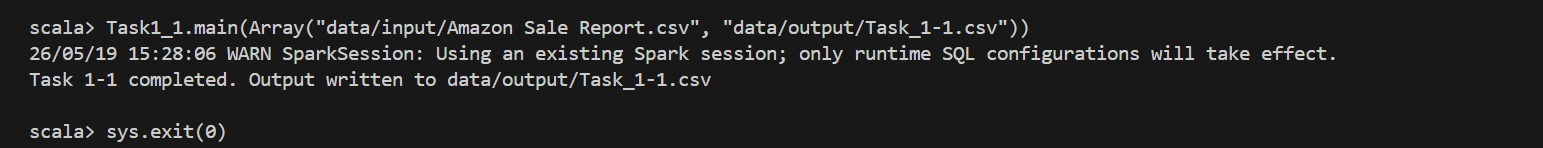
\includegraphics[width=0.9\textwidth]{img/1-1/run_success.png}
    \caption{Kết quả chạy chương trình Task 1.1}
    \label{fig:task1_1_run_success}
\end{figure}

\begin{figure}[H]
    \centering
    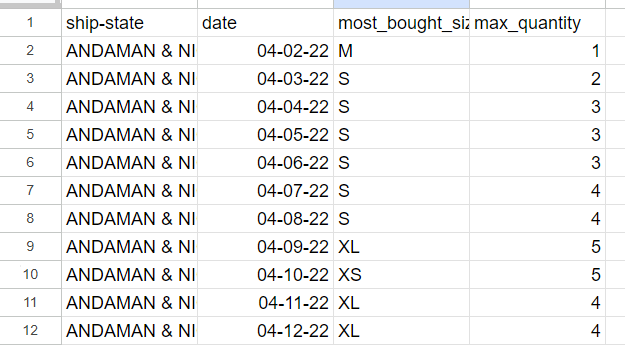
\includegraphics[width=0.9\textwidth]{img/1-1/output_preview.png}
    \caption{Một phần nội dung file \texttt{Task\_1-1.csv}}
    \label{fig:task1_1_output_preview}
\end{figure}

\begin{figure}[H]
    \centering
    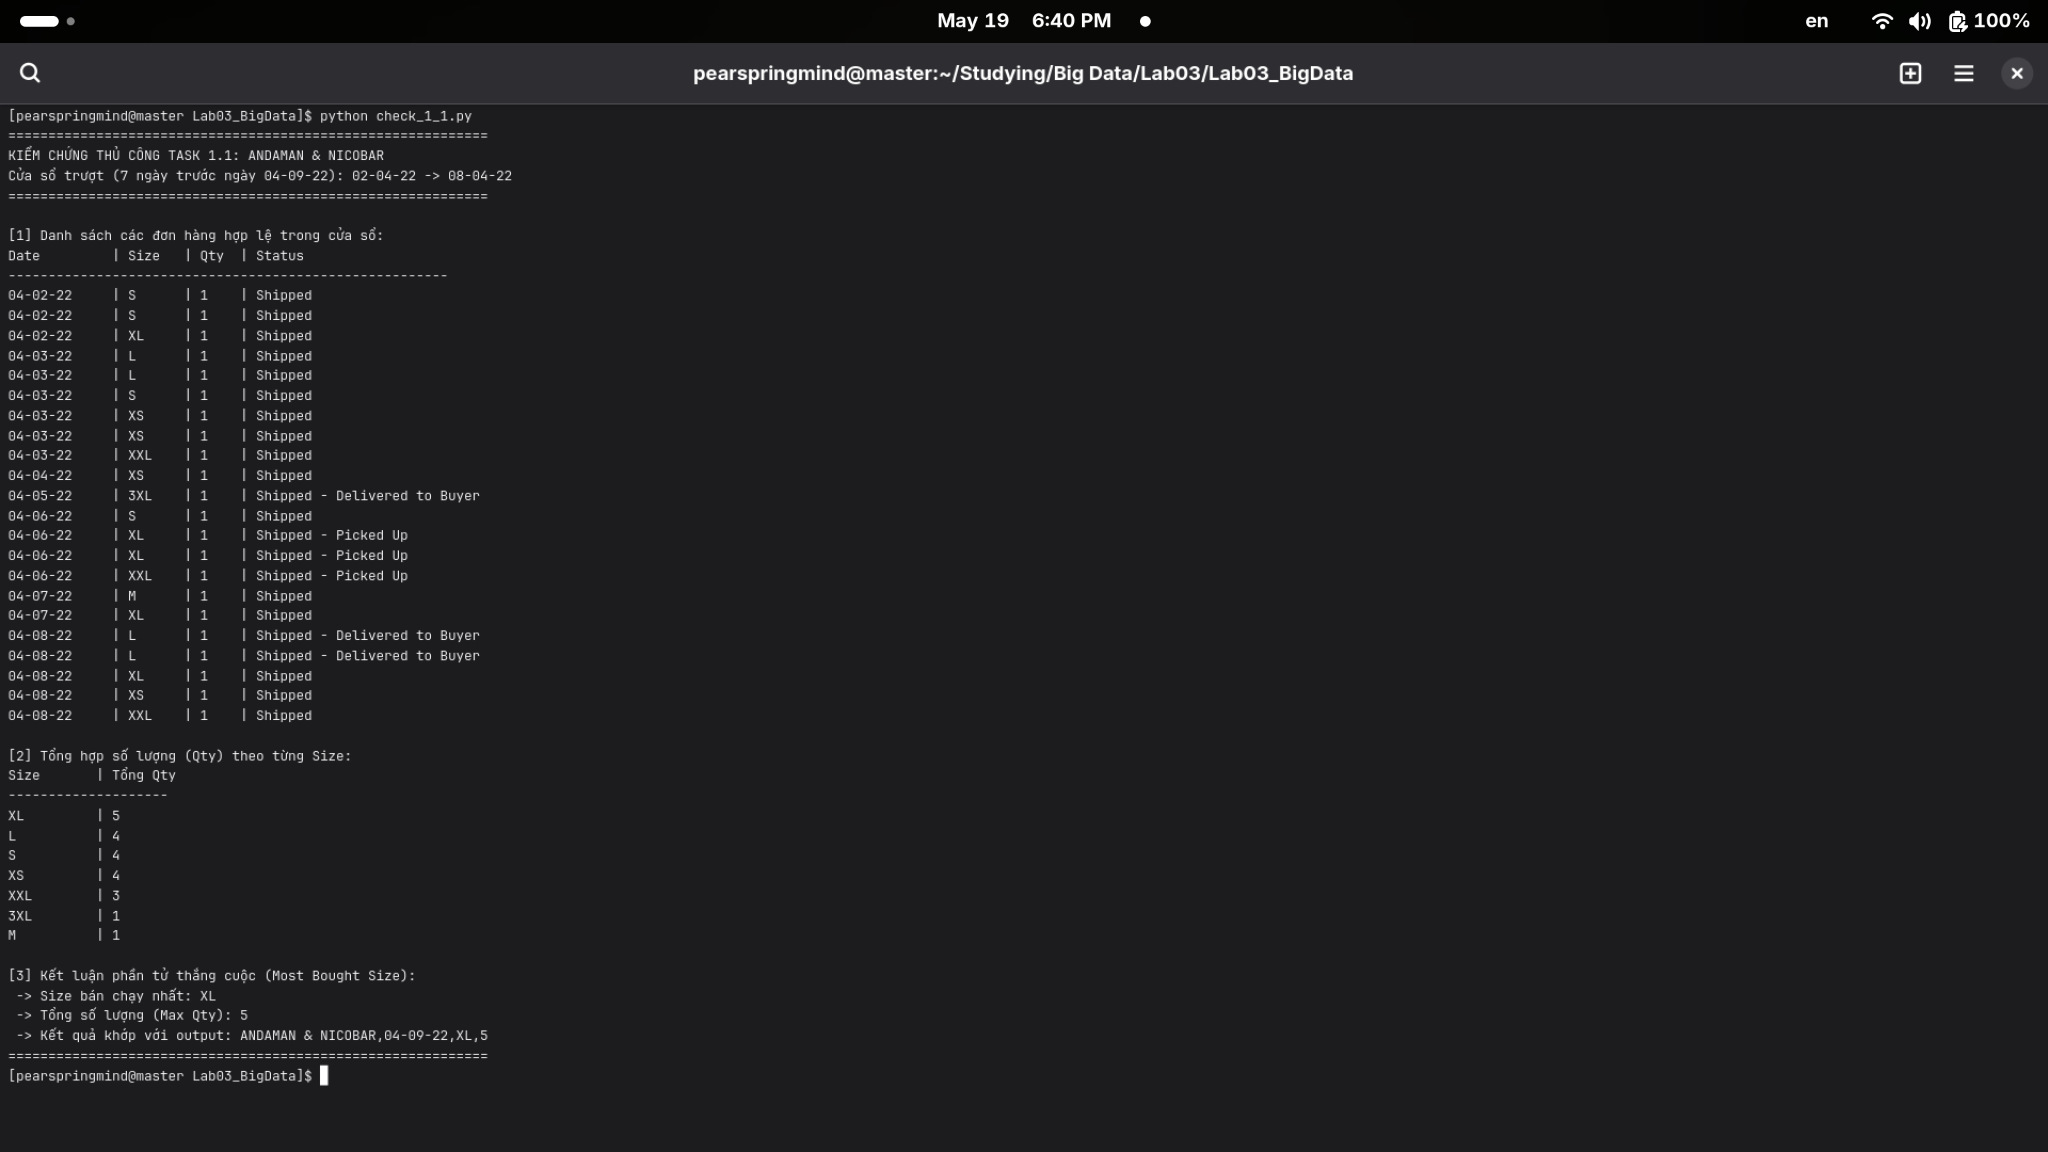
\includegraphics[width=0.9\textwidth]{img/1-1/manual_check.png}
    \caption{Kiểm chứng thủ công sliding window cho một state-date mẫu}
    \label{fig:task1_1_manual_check}
\end{figure}


%================================================
% TASK 1.2
%================================================
\section{Task 1.2: State-level Median Variety per Month}

\subsection*{Hướng dẫn điền nhanh cho người phụ trách}
Người phụ trách Task 1.2 cần điền đủ bốn nhóm nội dung: cách hiểu truy vấn, phân rã MapReduce, chiến lược triển khai bằng Scala, và kết quả kiểm chứng. Không cần viết lại đề bài dài; chỉ cần mô tả cách nhóm hiểu và cách code hiện thực hóa yêu cầu.

\begin{itemize}
    \item Điền đúng file nguồn: \texttt{src/Task\_1-2/src/main/scala/Task1\_2.scala}.
    \item Điền lệnh chạy thực tế đã dùng để tạo \texttt{data/output/Task\_1-2.csv}.
    \item Điền số dòng output, vài dòng mẫu, và một ví dụ kiểm chứng thủ công.
    \item Thêm ảnh vào thư mục \texttt{img/1-2} theo các tên gợi ý ở cuối section.
\end{itemize}

\subsection{Phân tích truy vấn (Query Analysis)}
\textbf{Mục tiêu cần viết.} Trình bày rằng với mỗi \texttt{ship-state} và mỗi tháng, ta cần tính median của ``variety'' trên các style thỏa điều kiện đã phục vụ ít nhất một size từ XXL trở lên.

\textbf{Cần định nghĩa rõ variety.} Ghi chính xác: variety của một style trong phạm vi \texttt{(state, month)} là số lượng \texttt{SKU} phân biệt của style đó trong cùng phạm vi. Nhấn mạnh variety không phải số order và không phải số size.

\textbf{Cần định nghĩa style qualify.} Ghi rõ style qualify nếu trong cùng \texttt{(state, month, style)} có ít nhất một record có size từ XXL trở lên. Nêu danh sách size code hỗ trợ trong code, ví dụ \texttt{XXL}, \texttt{2XL}, \texttt{XXXL}, \texttt{3XL}, \texttt{4XL}, \texttt{5XL}, \texttt{6XL}. Nếu code có regex cho các size lớn hơn, mô tả thêm.

\textbf{Điểm dễ sai cần giải thích.} Sau khi style qualify, variety vẫn phải đếm tất cả SKU của style trong tháng và state đó, kể cả SKU size nhỏ hơn XXL. Điều kiện XXL chỉ dùng để quyết định style có được đưa vào tập tính median hay không.

\textbf{Median cần ghi.} Mô tả cách tính median: nếu số style lẻ thì lấy phần tử giữa sau khi sort; nếu chẵn thì lấy trung bình hai phần tử giữa. Ghi rõ output làm tròn bao nhiêu chữ số thập phân nếu có.

\textbf{Schema cần điền.} Điền schema cuối cùng của \texttt{Task\_1-2.csv}:
\begin{itemize}
    \item \texttt{ship-state}: state đã chuẩn hóa theo code.
    \item \texttt{month}: định dạng tháng, ví dụ \texttt{YYYY-MM}.
    \item \texttt{median\_variety}: median variety của các qualifying styles.
\end{itemize}

\subsection{Phân rã thành các bước cơ bản (Decomposition)}
Điền theo cấu trúc dưới đây, mỗi bước nên có 2--4 câu: bước làm gì, key/value là gì, và vì sao cần bước đó.

\begin{enumerate}
    \item \textbf{Đọc input và chọn cột.} Ghi các cột dùng: \texttt{Date}, \texttt{SKU}, \texttt{Style}, \texttt{Size}, \texttt{ship-state}. Nêu cách drop null, trim chuỗi và parse tháng.
    \item \textbf{Map sang khóa style.} Ghi key là \texttt{(state, month, style)}, value là \texttt{(SKU, isAtLeastXXL)}.
    \item \textbf{Reduce lần 1 để tính variety và cờ XXL.} Ghi cách gom \texttt{SKU} vào set để đếm distinct, đồng thời OR các giá trị \texttt{isAtLeastXXL} thành \texttt{hasXXL}.
    \item \textbf{Lọc style qualify.} Ghi chỉ giữ style có \texttt{hasXXL = true}; đây là điều kiện của đề bài.
    \item \textbf{Map sang khóa state-month.} Ghi key là \texttt{(state, month)}, value là \texttt{variety} của style.
    \item \textbf{Reduce lần 2 để tính median.} Ghi cách gom list variety, sort tăng dần và tính median.
    \item \textbf{Xuất CSV.} Ghi cách sort output, ghi header và đảm bảo tạo một file CSV thường, không phải thư mục part files.
\end{enumerate}

\subsection{Lý do phân rã}
Viết đoạn giải thích vì sao phải tách ``qualify style'' và ``variety''. Gợi ý nội dung: cùng một style có thể có SKU size nhỏ và size lớn; nếu lọc chỉ còn dòng size XXL trước khi đếm variety thì sẽ làm mất SKU size nhỏ và sai định nghĩa variety. Vì vậy reducer đầu tiên phải vừa giữ tập SKU đầy đủ vừa ghi nhận style có từng phục vụ size từ XXL trở lên.

Viết thêm 1 đoạn về MapReduce: bài toán được quy về hai tầng aggregation. Tầng đầu xử lý ở cấp style; tầng thứ hai xử lý ở cấp state-month để tính median. Cách này phù hợp với key-value processing vì mỗi reducer chỉ cần dữ liệu cùng key.

\subsection{Chiến lược thực thi \& Triển khai mã nguồn}
\textbf{Điền lệnh chạy.}
\begin{lstlisting}[language=bash]
TODO: Điền lệnh chạy Task 1.2 thực tế.
\end{lstlisting}

\textbf{Điền snippet size threshold.} Chèn hàm hoặc đoạn code xác định \texttt{isAtLeastXXL}. Sau snippet, giải thích mapping size và regex nếu có.

\textbf{Điền snippet map/reduce variety.} Chèn đoạn code emit \texttt{((state, month, style), (sku, isXXL))} và đoạn \texttt{aggregateByKey}/\texttt{reduceByKey} dùng set SKU.

\textbf{Điền snippet median.} Chèn hàm \texttt{computeMedian} hoặc đoạn sort list variety và tính median.

\textbf{Điền xử lý dữ liệu lỗi.} Ghi cách code xử lý date parse lỗi, null, empty \texttt{SKU}/\texttt{Style}/\texttt{ship-state}, và vì sao cách đó không làm sai output.

\subsection{Kết quả thực thi \& Xuất dữ liệu}
\textbf{Điền thông tin output.}
\begin{itemize}
    \item Đường dẫn output: \texttt{data/output/Task\_1-2.csv}.
    \item Số dòng bao gồm header: TODO.
    \item Số dòng kết quả không tính header: TODO.
    \item Kích thước file: TODO.
\end{itemize}

\textbf{Điền sample output.}
\begin{lstlisting}[language={}]
TODO: Dán 5-10 dòng đầu của Task_1-2.csv.
\end{lstlisting}

\textbf{Điền kiểm chứng thủ công.} Chọn một \texttt{state-month} có ít nhất vài style. Tạo bảng gồm \texttt{style}, danh sách SKU distinct hoặc số SKU distinct, có size từ XXL trở lên hay không, variety. Sau đó sort các variety của style qualify và tính median để đối chiếu với output.

\subsection{Minh chứng bằng hình ảnh}
Thêm ảnh vào thư mục \texttt{img/1-2} theo các tên sau. Nếu chưa thêm ảnh, LaTeX sẽ hiển thị khung nhắc.

\begin{figure}[H]
    \centering
    \IfFileExists{img/1-2/run_success.png}
    {
\includegraphics[width=0.9\textwidth]{img/1-2/run_success.png}}
    {\fbox{\parbox[c][4cm][c]{0.85\textwidth}{\centering Thêm ảnh chạy thành công tại \texttt{img/1-2/run\_success.png}}}}
    \caption{Kết quả chạy chương trình Task 1.2}
\end{figure}

\begin{figure}[H]
    \centering
    \IfFileExists{img/1-2/output_preview.png}
    {
\includegraphics[width=0.9\textwidth]{img/1-2/output_preview.png}}
    {\fbox{\parbox[c][4cm][c]{0.85\textwidth}{\centering Thêm ảnh preview output tại \texttt{img/1-2/output\_preview.png}}}}
    \caption{Một phần nội dung file \texttt{Task\_1-2.csv}}
\end{figure}

\begin{figure}[H]
    \centering
    \IfFileExists{img/1-2/manual_check.png}
    {
\includegraphics[width=0.9\textwidth]{img/1-2/manual_check.png}}
    {\fbox{\parbox[c][4cm][c]{0.85\textwidth}{\centering Thêm ảnh kiểm chứng thủ công tại \texttt{img/1-2/manual\_check.png}}}}
    \caption{Kiểm chứng thủ công median variety cho một state-month mẫu}
\end{figure}


%================================================
% TASK 2.1
%================================================
\section{Task 2.1: Percentage of Cancelled Orders per City}

\subsection{Phân tích truy vấn}

Bài toán yêu cầu tính \textbf{phần trăm đơn hàng bị hủy} theo từng thành phố (\texttt{ship-city}), trong đó chỉ xét các đơn hàng thỏa mãn \textbf{đồng thời ba điều kiện} sau:

\textbf{Điều kiện 1 --- Mức dịch vụ.}
Đơn hàng phải có mức dịch vụ giao hàng \texttt{ship-service-level} bằng \texttt{"Standard"}. Trong mã nguồn, phép so sánh được chuẩn hóa bằng \texttt{lower(trim(col("ship-service-level"))) === "standard"} để tránh sai lệch do khoảng trắng thừa hoặc khác biệt giữa chữ hoa và chữ thường.

\textbf{Điều kiện 2 --- Có ít nhất 3 khuyến mãi hợp lệ về mặt thời gian.}
Mỗi đơn hàng chứa cột \texttt{promotion-ids}, là chuỗi các mã khuyến mãi được phân tách bằng dấu phẩy. Một chương trình khuyến mãi được gọi là \textit{hợp lệ về mặt thời gian} nếu khoảng thời gian hoạt động của nó trên \textbf{toàn bộ tập dữ liệu} kéo dài ít nhất 2 ngày. Cụ thể, với mỗi mã khuyến mãi duy nhất xuất hiện trong bộ dữ liệu:
\begin{itemize}
    \item Xác định ngày xuất hiện \textbf{đầu tiên} ($d_{\min}$) và ngày xuất hiện \textbf{cuối cùng} ($d_{\max}$).
    \item Tính khoảng thời gian hoạt động: $\text{active\_days} = d_{\max} - d_{\min}$ (tính bằng số ngày).
    \item Khuyến mãi hợp lệ khi và chỉ khi $\text{active\_days} \geq 2$.
\end{itemize}
Một đơn hàng thỏa mãn điều kiện này nếu trong danh sách \texttt{promotion-ids} của nó chứa \textbf{ít nhất 3} mã khuyến mãi hợp lệ, kể cả các khuyến mãi do Amazon phát hành.

\textbf{Điều kiện 3 --- Giá trị đơn hàng (Amount) thấp hơn mức trung bình của bang.}
Tính giá trị trung bình cột \texttt{Amount} theo từng bang \texttt{ship-state} trên tập con các đơn hàng thỏa mãn \texttt{Fulfilment = "Merchant"} và \texttt{Courier Status = "Shipped"}. Đơn hàng đang xét chỉ được giữ lại nếu:
\[
\texttt{Amount}_{\text{order}} < \overline{\texttt{Amount}}_{\text{Merchant,Shipped}}^{\text{(cùng bang)}}
\]

\textbf{Tính phần trăm đơn hàng bị hủy.}
Sau khi lọc ra tất cả đơn hàng thỏa mãn đồng thời cả ba điều kiện trên, chương trình tiến hành gom nhóm theo thành phố \texttt{ship-city} đã được chuẩn hóa để tính toán:
\[
\texttt{cancelled\_percentage} = \frac{|\{o : \texttt{Status}(o) = \text{``Cancelled''}\}|}{|\text{tổng số đơn hàng hợp lệ}|} \times 100
\]
Mã nguồn xác định trạng thái đơn hàng bị hủy bằng phép so khớp \texttt{lower(trim(col("Status"))) === "cancelled"} để đảm bảo tính chính xác sau khi chuẩn hóa.

\textbf{Cấu trúc dữ liệu đầu ra:}
\begin{table}[H]
\centering
\begin{tabular}{lll}
\toprule
\textbf{Cột} & \textbf{Kiểu} & \textbf{Ý nghĩa} \\
\midrule
\texttt{ship-city}  & String & Thành phố giao hàng đã chuẩn hóa viết hoa \\
\texttt{cancelled\_percentage} & Double & Tỷ lệ hủy (\%), làm tròn 4 chữ số thập phân \\
\bottomrule
\end{tabular}
\caption{Định nghĩa schema tệp đầu ra Task\_2-1.parquet}
\label{tab:task2_1_schema}
\end{table}

% ------------------------------------------------------------------
\subsection{Phân rã thành các bước cơ bản}

Lời giải được phân rã thành 9 bước xử lý tuần tự, mỗi bước tương ứng với một phép biến đổi DataFrame rõ ràng:

\begin{enumerate}
    \item \textbf{Đọc dữ liệu CSV và chuyển kiểu dữ liệu} (\texttt{df}).
    Đọc tệp CSV với dòng đầu chứa tiêu đề, tắt tính năng tự động suy luận kiểu dữ liệu (\texttt{inferSchema}) để kiểm soát kiểu dữ liệu một cách chủ động. Phân tích cột \texttt{Date} sang kiểu ngày (\texttt{date}) theo định dạng \texttt{MM-dd-yy}, chuyển kiểu cột \texttt{Amount} sang \texttt{DoubleType}, chuẩn hóa tên thành phố \texttt{ship-city} và bang \texttt{ship-state} bằng hàm \texttt{upper(trim(...))}, đồng thời tạo cột định danh \texttt{order\_row\_id} bằng hàm \texttt{monotonically\_increasing\_id()} để định danh duy nhất cho từng đơn hàng sau các phép liên kết. DataFrame này được lưu tạm vào bộ nhớ (\texttt{cache()}) vì sẽ được tái sử dụng trong nhiều nhánh xử lý khác nhau.

    \item \textbf{Tách các mã khuyến mãi thành từng dòng riêng} (\texttt{promoExploded}).
    Lọc bỏ các dòng có cột \texttt{promotion-ids} rỗng hoặc mang giá trị null. Sử dụng hàm \texttt{split} để tách chuỗi khuyến mãi theo dấu phẩy, dùng hàm \texttt{transform} kết hợp với \texttt{trim} để loại bỏ khoảng trắng dư thừa của từng mã, sau đó dùng hàm \texttt{explode} để phân rã danh sách thành từng dòng mã khuyến mãi riêng lẻ. Bước này rất quan trọng vì khoảng thời gian hoạt động là thuộc tính mang tính chất toàn cục của từng mã khuyến mãi — cần thu thập toàn bộ các ngày xuất hiện của mã trên toàn bộ tập dữ liệu.

    \item \textbf{Tính toán thời gian hợp lệ của khuyến mãi} (\texttt{promoValidity}).
    Gom nhóm theo mã khuyến mãi \texttt{promo\_id}, tính ngày xuất hiện sớm nhất \texttt{min(parsed\_date)} và muộn nhất \texttt{max(parsed\_date)}, sau đó sử dụng hàm hiệu ngày \texttt{datediff} để tính số ngày hoạt động \texttt{active\_days}. Chỉ giữ lại các mã khuyến mãi có số ngày hoạt động $\text{active\_days} \geq 2$.

    \item \textbf{Đếm số khuyến mãi hợp lệ theo từng đơn hàng bằng DataFrame}.
    Từ DataFrame gốc \texttt{df}, chương trình thực hiện phân rã các mã khuyến mãi theo định danh đơn hàng \texttt{order\_row\_id}, liên kết với bảng khuyến mãi hợp lệ \texttt{promoValidity}, sau đó gom nhóm theo \texttt{order\_row\_id} để đếm số lượng khuyến mãi hợp lệ duy nhất bằng hàm \texttt{countDistinct}. Cách làm này giữ nguyên tính chất declarative của Structured API, không sử dụng hàm tự định nghĩa (UDF) và không phải thu thập dữ liệu về nút điều phối, giúp Catalyst dễ dàng tối ưu hóa.

    \item \textbf{Áp dụng Điều kiện 1 và 2} (\texttt{afterCond12}).
    Lọc các đơn hàng có \texttt{ship-service-level = "Standard"}, sau đó thực hiện phép liên kết trái với bảng đếm số khuyến mãi hợp lệ \texttt{validPromotionCounts} theo \texttt{order\_row\_id}; các đơn hàng không có khuyến mãi nào hợp lệ sẽ nhận giá trị mặc định là \texttt{0} thông qua hàm \texttt{coalesce}. Cuối cùng, thực hiện lọc lấy các đơn hàng có \texttt{valid\_promo\_count >= 3}.

    \item \textbf{Tính toán giá trị trung bình Amount theo bang} (\texttt{stateAvgDf}).
    Từ DataFrame gốc \texttt{df} (không phải \texttt{afterCond12}), lọc các bản ghi có \texttt{Fulfilment = "Merchant"} và \texttt{Courier Status = "Shipped"}, loại bỏ các dòng có giá trị Amount bị null, sau đó thực hiện gom nhóm và tính trung bình: \texttt{groupBy("ship\_state\_norm").agg(avg("Amount"))}. Kết quả thu được là một bảng dữ liệu nhỏ chứa ngưỡng chi tiêu trung bình cho từng bang.

    \item \textbf{Liên kết và áp dụng Điều kiện 3} (\texttt{qualifiedDf}).
    Thực hiện phép liên kết trong giữa \texttt{afterCond12} và \texttt{stateAvgDf} trên cột bang \texttt{ship\_state\_norm}, sau đó lọc lấy các đơn hàng có \texttt{Amount < merchant\_shipped\_avg}. Sau bước này, ta thu được tập hợp các đơn hàng thỏa mãn đồng thời cả ba điều kiện lọc.

    \item \textbf{Tính phần trăm đơn hàng bị hủy theo từng thành phố} (\texttt{resultDf}).
    Gom nhóm theo thành phố \texttt{ship\_city\_norm}, đếm tổng số đơn hàng bằng \texttt{count(*)} và đếm số đơn hàng bị hủy bằng hàm tổng điều kiện \texttt{sum(when(... === "cancelled", 1).otherwise(0))}. Tính tỷ lệ phần trăm đơn hàng bị hủy và làm tròn đến 4 chữ số thập phân.

    \item \textbf{Xuất tệp Parquet duy nhất}.
    Sử dụng \texttt{coalesce(1)} để gom dữ liệu về một phân vùng duy nhất, ghi vào một thư mục tạm trên ổ đĩa, sau đó đổi tên tệp bộ phận thành tên tệp Parquet đơn lẻ chính xác theo đường dẫn đầu ra và dọn dẹp các tệp phụ checksum.
\end{enumerate}

% ------------------------------------------------------------------
\subsection{Lý do phân rã}

\textbf{Tính khoảng hoạt động hợp lệ của khuyến mãi trên toàn bộ tập dữ liệu trước.}
Khoảng thời gian hoạt động của một mã khuyến mãi được xác định bởi khoảng cách giữa ngày xuất hiện đầu tiên và ngày xuất hiện cuối cùng của nó trên toàn bộ tập dữ liệu, chứ không thể chỉ xét riêng lẻ trong từng đơn hàng. Do đó, quy trình phân rã-gom nhóm-hiệu ngày bắt buộc phải được xử lý trên toàn bộ dữ liệu trước khi áp dụng ngược lại cho từng đơn hàng. Đây là lý do quy trình xử lý được chia thành hai nhánh song song: một nhánh tính toán độ hợp lệ của các mã khuyến mãi và nhánh chính xử lý dữ liệu đơn hàng.

\textbf{Ngưỡng chi tiêu trung bình theo bang phải được tính riêng rồi liên kết sau.}
Điều kiện thứ ba yêu cầu so sánh giá trị \texttt{Amount} của mỗi đơn hàng với mức trung bình của bang tương ứng nhưng chỉ trên tập hợp con các đơn hàng của Merchant và đã Shipped. Vì tập hợp con này có tính chất khác biệt hoàn toàn với tập hợp đơn hàng Standard đang xét, chúng ta không thể sử dụng trực tiếp hàm cửa sổ mà bắt buộc phải tính toán trung bình riêng biệt thành bảng \texttt{stateAvgDf} rồi thực hiện phép liên kết theo cột \texttt{ship\_state\_norm}. Vì bảng \texttt{stateAvgDf} có kích thước rất nhỏ, Spark có thể tự động áp dụng phép liên kết phát tán \texttt{BroadcastHashJoin} để tránh chi phí phân tán dữ liệu qua mạng.

\textbf{Thứ tự áp dụng các điều kiện lọc giúp tối ưu hóa chi phí shuffle.}
Mã nguồn chủ động áp dụng Điều kiện 1 (lọc các đơn Standard) trước khi liên kết với bảng đếm số khuyến mãi để giảm thiểu số lượng đơn hàng tham gia vào phép liên kết. Điều kiện 3 (so sánh giá trị trung bình của bang) được áp dụng sau cùng vì nó phụ thuộc vào kết quả liên kết với bảng \texttt{stateAvgDf}. Nếu đảo ngược thứ tự — liên kết với bảng trung bình của bang trước rồi mới lọc mức dịch vụ và khuyến mãi — khối lượng dữ liệu tham gia vào phép liên kết và chi phí shuffle trung gian sẽ tăng lên rất nhiều.

% ------------------------------------------------------------------
\subsection{Chiến lược thực thi \& Triển khai mã nguồn}

Task 2.1 được cài đặt trong file \texttt{src/Task\_2-1/source/Task2\_1.scala}, sử dụng hoàn toàn DataFrame/Dataset API --- tuyệt đối không dùng các chuỗi truy vấn Spark SQL dạng thô. Chương trình nhận hai tham số: đường dẫn CSV đầu vào và đường dẫn file Parquet đầu ra.

\textbf{Lệnh chạy mẫu:}
\begin{lstlisting}[language=bash]
cat > /tmp/task2_1.runner.scala <<'EOF'
:load src/Task_2-1/source/Task2_1.scala
Task2_1.main(Array("data/input/Amazon Sale Report.csv",
  "data/output/Task_2-1.parquet"))
sys.exit(0)
EOF
spark-shell < /tmp/task2_1.runner.scala
\end{lstlisting}

\textbf{Explode và tính promotion validity.}
\begin{lstlisting}[language=Scala]
val promoExploded = df
  .filter(col("promotion-ids").isNotNull
       && col("promotion-ids") =!= "")
  .select(col("parsed_date"),
    explode(transform(
      split(col("promotion-ids"), ","),
      (promoId: Column) => trim(promoId)
    )).as("promo_id"))
  .filter(col("promo_id") =!= "")

val promoValidity = promoExploded
  .groupBy("promo_id")
  .agg(min("parsed_date").as("first_date"),
       max("parsed_date").as("last_date"))
  .withColumn("active_days",
    datediff(col("last_date"), col("first_date")))
  .filter(col("active_days") >= 2)
  .select("promo_id")
\end{lstlisting}

Lý do chương trình sử dụng hàm biến đổi \texttt{transform} kết hợp với \texttt{trim} trước khi chạy \texttt{explode} thay vì cắt khoảng trắng sau khi phân rã là: đảm bảo mỗi mã khuyến mãi được làm sạch ngay trong mảng trước khi phân rã dòng mới, tránh sinh ra các dòng trống vô nghĩa do các dấu phẩy dư thừa ở cuối chuỗi.

\textbf{Đếm valid promotions theo order bằng DataFrame.}
\begin{lstlisting}[language=Scala]
val orderPromos = df
  .filter(col("promotion-ids").isNotNull &&
          trim(col("promotion-ids")) =!= "")
  .select(col("order_row_id"),
    explode(transform(split(col("promotion-ids"), ","),
      (promoId: Column) => trim(promoId))).as("promo_id"))
  .filter(col("promo_id") =!= "")

val validPromotionCounts = orderPromos
  .join(broadcast(promoValidity), Seq("promo_id"), "inner")
  .groupBy("order_row_id")
  .agg(countDistinct("promo_id").as("valid_promo_count"))
\end{lstlisting}

Chiến lược này giữ trọn vẹn tính chất declarative của Structured API. Bảng \texttt{promoValidity} chỉ chứa 185 khuyến mãi hợp lệ nên được Spark tự động phát tán làm nhánh dựng bảng \textbf{Build side} khi liên kết với \texttt{orderPromos}; phần đếm số lượng theo khóa \texttt{order\_row\_id} là phép gom nhóm rõ ràng, hiển thị trực quan trong kế hoạch vật lý.

\textbf{Filter service level và đếm promotions.}
\begin{lstlisting}[language=Scala]
val afterCond12 = df
  .filter(lower(trim(
    col("ship-service-level"))) === "standard")
  .join(validPromotionCounts, Seq("order_row_id"), "left")
  .withColumn("valid_promo_count",
    coalesce(col("valid_promo_count"), lit(0L)))
  .filter(col("valid_promo_count") >= 3)
\end{lstlisting}

\textbf{Tính trung bình Amount theo state.}
\begin{lstlisting}[language=Scala]
val stateAvgDf = df
  .filter(
    lower(trim(col("Fulfilment"))) === "merchant" &&
    lower(trim(col("Courier Status"))) === "shipped")
  .filter(col("Amount").isNotNull)
  .groupBy("ship_state_norm")
  .agg(avg("Amount").as("merchant_shipped_avg"))
\end{lstlisting}

\textbf{Join điều kiện 3 và tính cancelled percentage.}
\begin{lstlisting}[language=Scala]
val joinedDf = afterCond12.join(
  stateAvgDf, Seq("ship_state_norm"), "inner")

val qualifiedDf = joinedDf
  .filter(col("Amount").isNotNull)
  .filter(col("Amount") < col("merchant_shipped_avg"))

val resultDf = qualifiedDf
  .groupBy(col("ship_city_norm"))
  .agg(
    count("*").as("total_orders"),
    sum(when(lower(trim(col("Status"))) === "cancelled",
             1).otherwise(0)).as("cancelled_orders"))
  .withColumn("cancelled_percentage",
    round(col("cancelled_orders") /
          col("total_orders") * 100.0, 4))
  .select(col("ship_city_norm").as("ship-city"),
          col("cancelled_percentage"))
  .orderBy("ship-city")
\end{lstlisting}

Việc chuẩn hóa tên thành phố \texttt{ship-city} trước khi gom nhóm là cực kỳ cần thiết để loại bỏ các sai lệch do chữ hoa/thường và khoảng trắng thừa. Kết quả cuối cùng bám sát yêu cầu của đề bài: tính tỷ lệ phần trăm cho từng thành phố.

% ------------------------------------------------------------------
\subsection{Phân tích chuyên sâu --- Kế hoạch thực thi}

\subsubsection{Đầu ra của lệnh explain(true)}
Dưới đây là kế hoạch thực thi chi tiết thu được từ lệnh \texttt{resultDf.explain(true)} khi chạy chương trình:

\begin{lstlisting}[language={},basicstyle=\ttfamily\tiny]
== Physical Plan ==
AdaptiveSparkPlan isFinalPlan=false
+- Sort [ship-city ASC NULLS FIRST], true, 0
   +- Exchange rangepartitioning(ship-city ASC NULLS FIRST, 200)
      +- HashAggregate(keys=[ship_city_norm], functions=[sum(...), count(1)])
         +- Exchange hashpartitioning(ship_city_norm, 200)
            +- HashAggregate(keys=[ship_city_norm], functions=[partial_sum(...), partial_count(1)])
               +- Project [Status, ship_city_norm]
                  +- BroadcastHashJoin [ship_state_norm], [ship_state_norm], Inner, BuildRight,
                     (Amount < merchant_shipped_avg), false
                     :- Project [Status, Amount, ship_city_norm, ship_state_norm]
                     :  +- BroadcastHashJoin [order_row_id], [order_row_id], Inner, BuildRight, false
                     :     :- Filter lower(trim(ship-service-level)) = standard
                     :     +- BroadcastExchange HashedRelationBroadcastMode(order_row_id)
                     :        +- Filter coalesce(valid_promo_count, 0) >= 3
                     :           +- HashAggregate(keys=[order_row_id],
                     :              functions=[count(distinct promo_id)])
                     :              +- Exchange hashpartitioning(order_row_id, 200)
                     :                 +- HashAggregate(keys=[order_row_id, promo_id])
                     :                    +- Exchange hashpartitioning(order_row_id, promo_id, 200)
                     :                       +- BroadcastHashJoin [promo_id], [promo_id],
                     :                          Inner, BuildRight, false
                     :                          :- Generate explode(transform(split(promotion-ids, ","), trim))
                     :                          +- BroadcastExchange HashedRelationBroadcastMode(promo_id)
                     :                             +- HashAggregate(keys=[promo_id],
                     :                                functions=[min(parsed_date), max(parsed_date)])
                     :                                +- Exchange hashpartitioning(promo_id, 200)
                     +- BroadcastExchange HashedRelationBroadcastMode(ship_state_norm)
                        +- HashAggregate(keys=[ship_state_norm], functions=[avg(Amount)])
                           +- Exchange hashpartitioning(ship_state_norm, 200)
\end{lstlisting}

\subsubsection{Phân tích chiến lược liên kết vật lý}

Quy trình xử lý chứa một phép liên kết chính: \texttt{afterCond12} $\bowtie_{\texttt{ship\_state\_norm}}$ \texttt{stateAvgDf}.

\begin{table}[H]
\centering
\begin{tabular}{p{4cm}lp{6cm}}
\toprule
\textbf{Join} & \textbf{Strategy thực tế} & \textbf{Giải thích} \\
\midrule
\texttt{orderPromos} $\bowtie$ \texttt{promoValidity} & BroadcastHashJoin & \texttt{promoValidity} chỉ có 185 dòng nên được broadcast làm build side. \\
\texttt{standardOrders} $\bowtie$ \texttt{validPromotionCounts} & BroadcastHashJoin & Bảng order đủ điều kiện promotion sau aggregation nhỏ hơn ngưỡng broadcast, Spark chọn BuildRight. \\
\texttt{afterCond12} $\bowtie$ \texttt{stateAvgDf} & BroadcastHashJoin & \texttt{stateAvgDf} chỉ có bảng trung bình theo state, nhỏ hơn nhiều so với broadcast threshold mặc định 10 MB. \\
\bottomrule
\end{tabular}
\caption{Chi tiết các phép liên kết trong kế hoạch thực thi vật lý}
\label{tab:task2_1_joins}
\end{table}

Nhánh dựng bảng \textbf{Build side} của cả ba phép liên kết phát tán \texttt{BroadcastHashJoin} đều nằm ở phía bên phải trong kế hoạch vật lý: \texttt{promoValidity}, \texttt{validPromotionCounts}, và \texttt{stateAvgDf}. Spark tiến hành tuần tự hóa các bảng nhỏ này, phát tán đến các nút thực thi, sau đó thực hiện tìm kiếm bảng băm cục bộ trên phân vùng của bảng lớn hơn. Nhờ đó, các phép liên kết chính không cần phải thực hiện phân tán lại dữ liệu cả hai phía theo khóa liên kết.

Nếu \texttt{stateAvgDf} vượt quá 10 MB (cấu hình mặc định \texttt{spark.sql.autoBroadcastJoinThreshold}), Spark sẽ chuyển sang phép liên kết \texttt{SortMergeJoin} --- yêu cầu shuffle cả hai bảng theo khóa liên kết --- tốn kém hiệu năng hơn rất nhiều. Trong trường hợp cụ thể này, bảng chỉ có $\sim$36 dòng nên BroadcastHashJoin là sự lựa chọn tối ưu nhất.

\subsubsection{Đếm các nút trao đổi dữ liệu}

Dựa trên kế hoạch vật lý thực tế, các nút trao đổi dữ liệu phân tán chính gồm có:

\begin{table}[H]
\centering
\begin{tabular}{clp{6.5cm}}
\toprule
\textbf{\#} & \textbf{Exchange} & \textbf{Mục đích} \\
\midrule
1 & \texttt{hashpartitioning(promo\_id)} & Gom ngày xuất hiện của từng promotion để tính min/max date. \\
2 & \texttt{hashpartitioning(order\_row\_id, promo\_id)} & Khử trùng lặp cặp order--promotion trước khi \texttt{countDistinct}. \\
3 & \texttt{hashpartitioning(order\_row\_id)} & Gom các promotion hợp lệ theo từng order. \\
4 & \texttt{hashpartitioning(ship\_state\_norm)} & Tính trung bình Amount cho Merchant+Shipped theo state. \\
5 & \texttt{hashpartitioning(ship\_city\_norm)} & Gom các đơn qualified theo city để tính percentage. \\
6 & \texttt{rangepartitioning(ship-city)} & Sort toàn cục output cuối. \\
\bottomrule
\end{tabular}
\caption{Phân tích các nút trao đổi dữ liệu và mục đích sử dụng}
\label{tab:task2_1_exchanges}
\end{table}

\textbf{Lưu ý:} Kế hoạch thực thi còn có các nút phát tán \texttt{BroadcastExchange} dành cho các bảng \texttt{promoValidity}, \texttt{validPromotionCounts} và \texttt{stateAvgDf}; đây là cơ chế phát tán bảng nhỏ, hoàn toàn khác với các phép shuffle phân tán dữ liệu của các bảng lớn.

\subsubsection{Đếm các giai đoạn thực thi}

Mỗi nút trao đổi dữ liệu shuffle Exchange sẽ tạo ra một ranh giới phân tách giai đoạn thực thi mới. Với 6 nút shuffle Exchange chính và 3 nút BroadcastExchange, quy trình xử lý kết quả cần khoảng \textbf{7--9 giai đoạn thực thi} cho hành động ghi kết quả đầu ra; số stage thực tế có thể thay đổi nhẹ tùy theo các hành động phụ như \texttt{count()} hay \texttt{show()} phục vụ việc ghi nhật ký.

\begin{enumerate}
    \item \textbf{Stage 1:} Đọc tệp CSV, phân tích ngày tháng và giá trị đơn hàng, duyệt toàn bộ dữ liệu đầu vào.
    \item \textbf{Stage 2:} Phân rã mã khuyến mãi, shuffle theo \texttt{promo\_id}, tính toán ngày bắt đầu và kết thúc.
    \item \textbf{Stage 3:} Lọc đơn hàng Merchant+Shipped, shuffle theo \texttt{ship\_state\_norm}, tính Amount trung bình.
    \item \textbf{Stage 4:} Phân rã khuyến mãi đơn hàng, liên kết phát tán với \texttt{promoValidity}, shuffle theo \texttt{order\_row\_id}.
    \item \textbf{Stage 5:} Lọc mức dịch vụ Standard, thực hiện phép liên kết BroadcastHashJoin với \texttt{validPromotionCounts}.
    \item \textbf{Stage 6:} Thực hiện phép liên kết BroadcastHashJoin với \texttt{stateAvgDf}, lọc giá trị đơn hàng hợp lệ.
    \item \textbf{Stage 7:} Shuffle dữ liệu theo \texttt{ship\_city\_norm}, tính tổng số đơn và đơn bị hủy.
    \item \textbf{Stage 8:} Sắp xếp toàn cục, gộp phân vùng và ghi dữ liệu ra định dạng Parquet.
\end{enumerate}

\subsubsection{Thảo luận về cơ chế tự thích ứng khi thực thi truy vấn}

Trong mã nguồn của Task 2.1, chương trình sử dụng cấu hình mặc định của Spark runtime cho cơ chế tự thích ứng AQE (\texttt{spark.sql.adaptive.enabled}). Với môi trường thực thi Spark 3.4.0, kế hoạch vật lý hiển thị từ khóa \texttt{AdaptiveSparkPlan}, xác nhận AQE đang hoạt động và có thể mang lại các tối ưu hóa sau:
\begin{itemize}
    \item \textbf{Tự động gộp phân vùng sau khi shuffle:} gộp các phân vùng nhỏ sau shuffle, giảm số lượng task dư thừa.
    \item \textbf{Tự động chuyển đổi phép liên kết SortMergeJoin sang BroadcastHashJoin:} nếu sau bước lọc dữ liệu, một bên của phép liên kết có kích thước nhỏ hơn ngưỡng quy định, AQE sẽ tự động chuyển đổi chiến lược liên kết để tối ưu hiệu năng.
    \item \textbf{Tối ưu hóa các phép liên kết bị lệch dữ liệu:} tự động chia nhỏ các phân vùng bị lệch dữ liệu lớn thành nhiều phân vùng nhỏ hơn. Trong quy trình này, phép liên kết trên bang \texttt{ship-state} ít bị ảnh hưởng bởi hiện tượng lệch dữ liệu vì mỗi bang chỉ chứa duy nhất một dòng kết quả trung bình.
\end{itemize}

Trong kế hoạch thực thi minh họa ở trên, dòng chữ \texttt{AdaptiveSparkPlan isFinalPlan=false} xuất hiện do lệnh \texttt{resultDf.explain(true)} được gọi trước khi thực thi hành động ghi dữ liệu đầu ra. Tại thời điểm đó, Spark mới chỉ hiển thị kế hoạch thích ứng ban đầu; AQE vẫn cần thu thập phản hồi trong lúc chạy từ các giai đoạn shuffle trước để đưa ra kế hoạch tối ưu cuối cùng sau khi hành động ghi được thực hiện. Vì vậy, trạng thái \texttt{isFinalPlan=false} hoàn toàn phản ánh đúng nguyên lý hoạt động của AQE.

% ------------------------------------------------------------------
\subsection{Kết quả thực thi \& Xuất dữ liệu}

\begin{itemize}
    \item \textbf{Đường dẫn đầu ra:} \texttt{data/output/Task\_2-1.parquet}.
    \item \textbf{Định dạng:} Tệp Parquet duy nhất, có thể đọc dễ dàng bằng thư viện Pandas (\texttt{pd.read\_parquet}) hoặc Spark ở chế độ chạy cục bộ.
    \item \textbf{Số dòng kết quả:} 2,452 nhóm thành phố.
    \item \textbf{Kích thước tệp:} phụ thuộc vào siêu dữ liệu Parquet của lần ghi dữ liệu thực tế.
\end{itemize}

\textbf{Bảng tổng hợp trích xuất từ tệp Parquet đầu ra:}
\begin{table}[H]
\centering
\begin{tabular}{lr}
\toprule
\textbf{Chỉ số} & \textbf{Giá trị} \\
\midrule
Số dòng kết quả đầu ra & 2,452 \\
Số thành phố duy nhất & 2,452 \\
Giá trị nhỏ nhất của \texttt{cancelled\_percentage} & 0.0 \\
Giá trị lớn nhất của \texttt{cancelled\_percentage} & 0.0 \\
Số thành phố có tỷ lệ đơn bị hủy \texttt{cancelled\_percentage > 0} & 0 \\
\bottomrule
\end{tabular}
\caption{Các chỉ số thống kê tổng quan trích xuất từ tệp Parquet đầu ra của Task 2.1}
\label{tab:task2_1_summary_metrics}
\end{table}

\textbf{Một số dòng kết quả mẫu:}
\begin{lstlisting}[language={}]
ship-city                                      cancelled_percentage
(CHIKMAGALUR DISTERICT).     (N.R PUR THALUKU) 0.0
7BARASAT                                      0.0
ABHAYAPURI                                    0.0
ABOHAR                                        0.0
ABU ROAD                                      0.0
ACHALPUR                                      0.0
ACHANTA                                       0.0
ADAJAN GAM, SURAT                             0.0
ADALAJ                                        0.0
ADBHAR                                        0.0
\end{lstlisting}

\textbf{Kiểm chứng thủ công.}
Chọn thành phố mẫu \texttt{ship-city = BENGALURU}. Sau khi áp dụng đủ ba điều kiện lọc của đề bài, truy vấn kiểm chứng thủ công thu được 1,318 đơn hàng hợp lệ, trong đó không có đơn hàng nào mang trạng thái bị hủy (\texttt{cancelled\_orders = 0}). Các dòng đơn hàng mẫu đều thỏa mãn các mức dịch vụ Standard, số khuyến mãi hợp lệ $\geq 3$ và giá trị đơn hàng nhỏ hơn mức trung bình của bang tương ứng. Do đó:
\[
\texttt{cancelled\_percentage} = \frac{0}{1318} \times 100 = 0.0000
\]
Giá trị này khớp hoàn toàn với kết quả đầu ra \texttt{BENGALURU, 0.0}. Toàn bộ tỷ lệ hủy trong lần chạy dữ liệu hiện tại đều bằng 0 vì không có đơn hàng hợp lệ nào mang trạng thái \texttt{Cancelled}.

% ------------------------------------------------------------------
\subsection{Minh chứng bằng hình ảnh}

Các hình ảnh dưới đây cung cấp minh chứng trực quan về việc chạy chương trình, kế hoạch thực thi Catalyst plan và kết quả kiểm tra tệp dữ liệu đầu ra của Task 2.1.

\begin{figure}[H]
    \centering
    
\includegraphics[width=0.9\textwidth]{img/2-1/run_success.png}
    \caption{Kết quả chạy chương trình Task 2.1}
    \label{fig:task2_1_run_success}
\end{figure}

\begin{figure}[H]
    \centering
    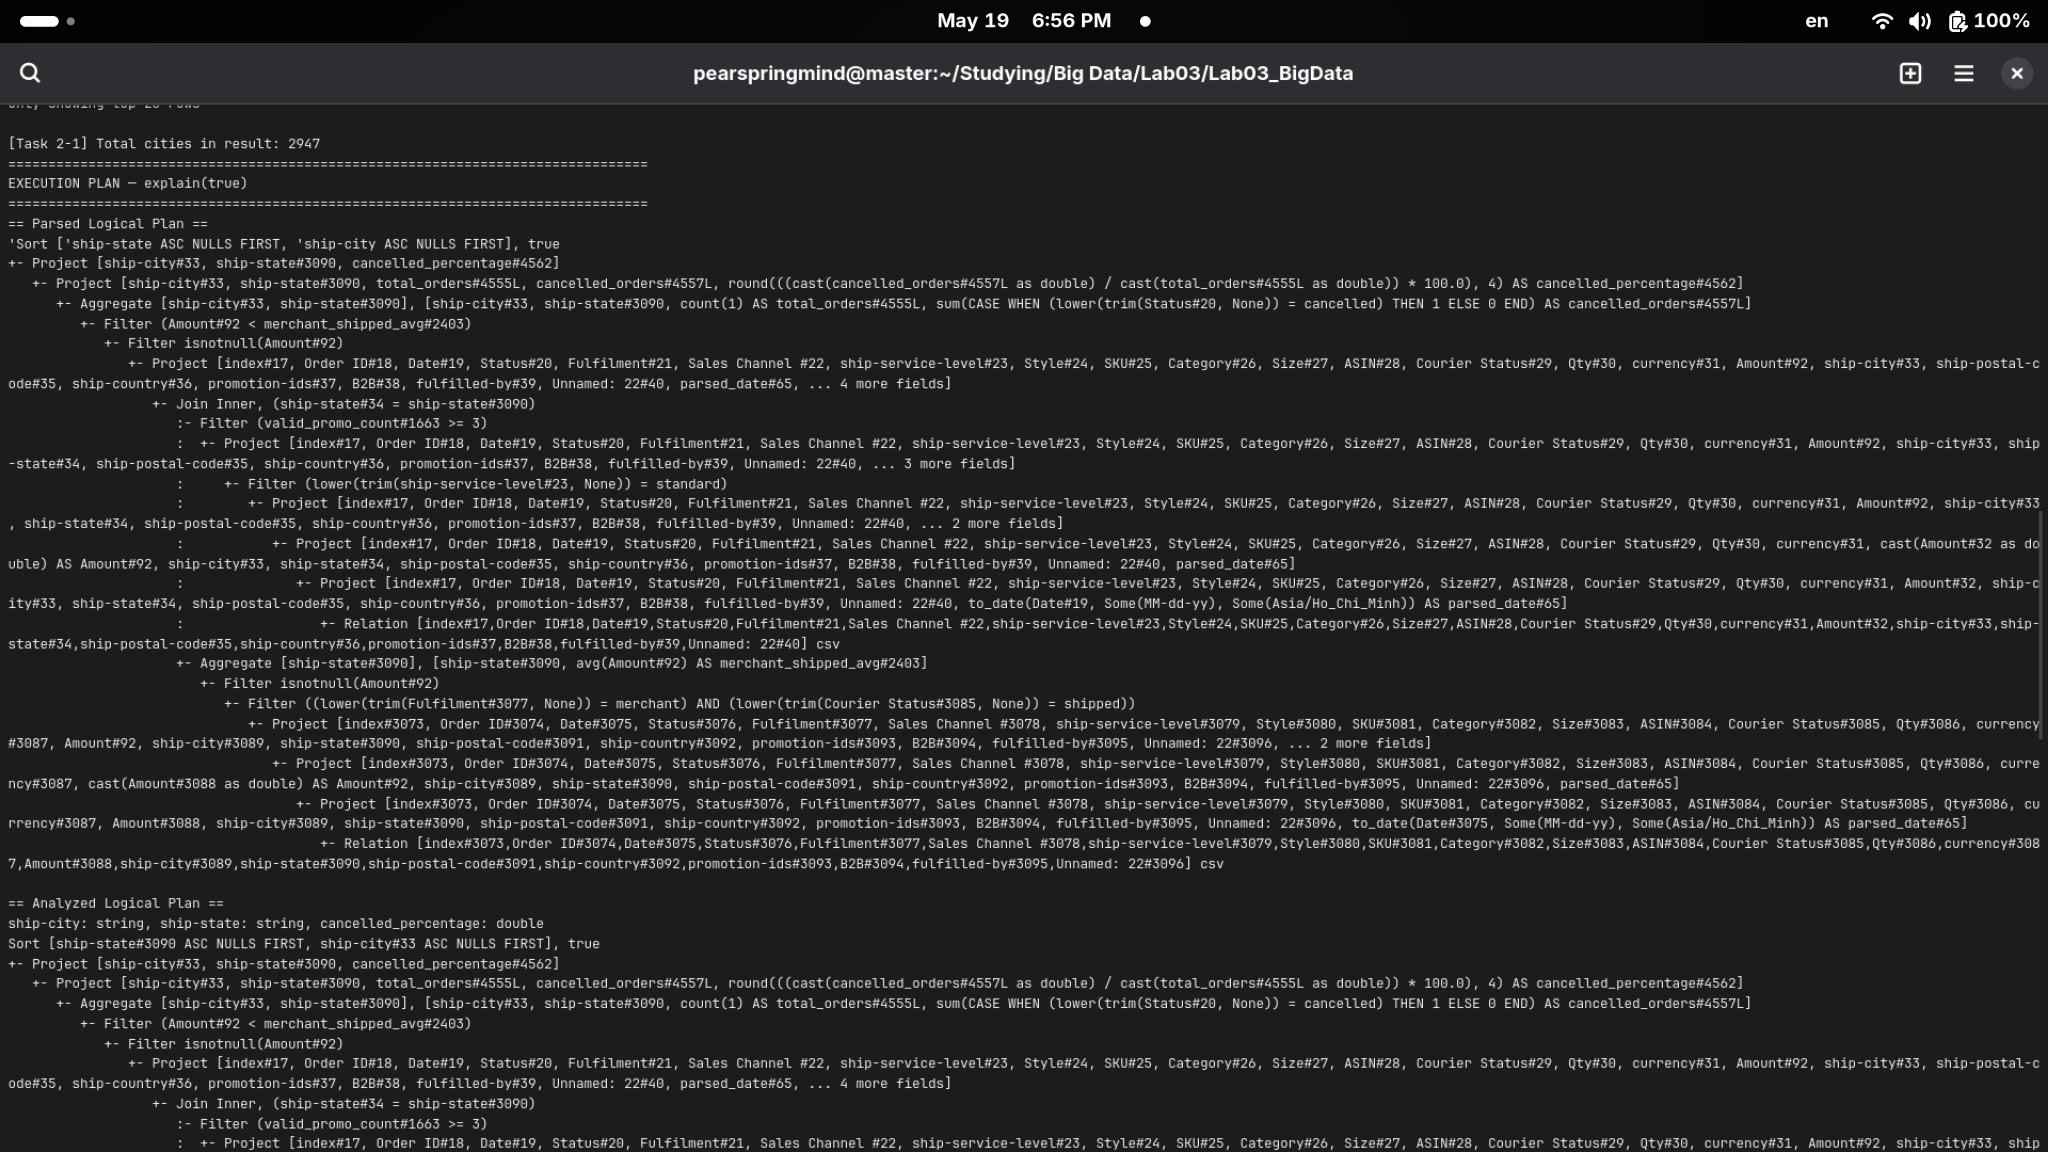
\includegraphics[width=0.9\textwidth]{img/2-1/explain_plan.png}
    \caption{Kế hoạch thực thi vật lý (Execution plan) của Task 2.1}
    \label{fig:task2_1_explain_plan}
\end{figure}

\begin{figure}[H]
    \centering
    
\includegraphics[width=0.9\textwidth]{img/2-1/output_preview.png}
    \caption{Một phần nội dung tệp Parquet kết quả đầu ra \texttt{Task\_2-1.parquet}}
    \label{fig:task2_1_output_preview}
\end{figure}


%================================================
% TASK 2.2
%================================================
\section{Task 2.2: StdDev of Amount by SKU-Month with Percentile Threshold}

\subsection{Phân tích truy vấn}
Task 2.2 được phụ trách bởi Nguyễn Hồ Anh Tuấn (23120185). Mục tiêu của truy vấn là xét từng nhóm cặp \texttt{(SKU, month)}, tìm các đơn hàng có số lượng khuyến mãi đủ lớn dựa theo ngưỡng phân vị động của chính nhóm đó, sau đó tính độ lệch chuẩn tổng thể của giá trị \texttt{Amount} trên tập các đơn hàng được giữ lại. Hai mức phân vị bắt buộc là P90 và P80.

Đơn vị lọc ở đây không phải là giá trị đơn hàng \texttt{Amount}, mà là số lượng khuyến mãi của từng đơn hàng. Cột \texttt{promotion-ids} được tách ra theo dấu phẩy, loại bỏ khoảng trắng thừa ở mỗi thành phần, bỏ qua các thành phần rỗng và đếm tất cả các mã khuyến mãi còn lại. Các chương trình khuyến mãi do Amazon phát hành vẫn được tính như khuyến mãi thông thường theo yêu cầu đề bài. Nếu cột \texttt{promotion-ids} mang giá trị null hoặc rỗng, số lượng khuyến mãi \texttt{promo\_count} của đơn hàng được đặt mặc định là 0.

Với mỗi nhóm \texttt{SKU-month}, chương trình tính hai ngưỡng động: \texttt{p90\_thresh} và \texttt{p80\_thresh}. Một đơn hàng được xem là hợp lệ cho mức P90 nếu \texttt{promo\_count >= p90\_thresh}; tương tự, hợp lệ cho P80 nếu \texttt{promo\_count >= p80\_thresh}. Ngưỡng này được tính toán riêng biệt cho từng nhóm cụ thể, hoàn toàn không sử dụng một ngưỡng chung cho toàn bộ tập dữ liệu.

Độ lệch chuẩn tổng thể được tính toán bằng hàm \texttt{stddev\_pop}, tức là độ lệch chuẩn tổng thể với bậc tự do bằng 0:
\[
    \sigma = \sqrt{\frac{\sum_{i=1}^{N}(x_i-\mu)^2}{N}}
\]
Nếu sau khi thực hiện lọc theo phân vị mà nhóm đó có ít hơn 2 đơn hàng, kết quả độ lệch chuẩn của nhóm sẽ được đặt mặc định là \texttt{0.0}. Quy tắc này giúp tránh việc diễn giải sai lệch cho các nhóm chỉ còn lại 0 hoặc 1 đơn hàng hợp lệ sau khi lọc.

Dữ liệu đầu ra được ghi dưới dạng một tệp Parquet duy nhất tại \texttt{data/output/Task\_2-2.parquet} với cấu trúc như sau:
\begin{table}[H]
\centering
\begin{tabular}{ll}
\toprule
\textbf{Cột} & \textbf{Ý nghĩa} \\
\midrule
\texttt{SKU} & Mã SKU của sản phẩm \\
\texttt{month} & Tháng theo định dạng \texttt{yyyy-MM} \\
\texttt{p90\_stddev\_approx} & Độ lệch chuẩn Amount khi dùng ngưỡng phân vị gần đúng P90 \\
\texttt{p90\_stddev\_exact} & Độ lệch chuẩn Amount khi dùng ngưỡng phân vị chính xác P90 \\
\texttt{p80\_stddev\_approx} & Độ lệch chuẩn Amount khi dùng ngưỡng phân vị gần đúng P80 \\
\texttt{p80\_stddev\_exact} & Độ lệch chuẩn Amount khi dùng ngưỡng phân vị chính xác P80 \\
\bottomrule
\end{tabular}
\caption{Định nghĩa schema tệp đầu ra Task\_2-2.parquet}
\label{tab:task2_2_schema}
\end{table}

\subsection{Phân rã thành các bước cơ bản}
Tệp mã nguồn của phần này là \texttt{src/Task\_2-2/source/Task2\_2.scala}. Toàn bộ lời giải sử dụng Spark Structured APIs bằng Scala, tuyệt đối không sử dụng các chuỗi truy vấn Spark SQL dạng thô.

\begin{enumerate}
    \item \textbf{Đọc dữ liệu CSV và chọn các cột cần thiết.} Chương trình đọc tệp dữ liệu \texttt{data/input/Amazon Sale Report.csv} có dòng đầu chứa tiêu đề, giữ lại các cột \texttt{SKU}, \texttt{Date}, \texttt{promotion-ids}, \texttt{Amount}. Cột \texttt{Amount} được chuyển kiểu sang \texttt{DoubleType}; các dòng thiếu thông tin \texttt{SKU}, thiếu ngày tháng hoặc không thể chuyển đổi giá trị \texttt{Amount} sẽ bị loại bỏ để đảm bảo tính hợp lệ cho phép tính độ lệch chuẩn sau này.
    \item \textbf{Chuẩn hóa định dạng tháng.} Cột \texttt{Date} được phân tích cú pháp bằng nhiều định dạng phổ biến như \texttt{M/d/yyyy}, \texttt{MM-dd-yy}, \texttt{M/d/yy}. Sau khi chuyển đổi thành kiểu ngày hợp lệ, chương trình tạo cột tháng \texttt{month = date\_format(parsed\_date, "yyyy-MM")}.
    \item \textbf{Tính số lượng khuyến mãi của đơn hàng} (\texttt{promo\_count}). Cột \texttt{promotion-ids} được tách theo dấu phẩy, loại bỏ khoảng trắng ở mỗi mã khuyến mãi và lọc bỏ các mã rỗng. Số lượng mã hợp lệ còn lại là \texttt{promo\_count}; nếu cột mang giá trị null hoặc rỗng thì mặc định đặt bằng 0.
    \item \textbf{Tạo DataFrame cơ sở.} DataFrame \texttt{baseDf} chỉ giữ lại các cột thông tin tối giản gồm \texttt{SKU}, \texttt{month}, \texttt{promo\_count}, \texttt{amount\_val}. DataFrame này được lưu tạm vào bộ nhớ (\texttt{cache()}) vì cả hai phương pháp tính phân vị gần đúng và chính xác đều sẽ tái sử dụng lại tập dữ liệu này.
    \item \textbf{Tính toán ngưỡng phân vị gần đúng} (\texttt{approxThresholds}). Gom nhóm theo cặp \texttt{SKU, month} và tính toán các ngưỡng phân vị P90 và P80 thông qua hàm \texttt{percentile\_approx(promo\_count, p, 10000)}. Ngưỡng này sau đó được liên kết ngược lại với DataFrame cơ sở \texttt{baseDf} để tiến hành lọc lấy các đơn hàng thỏa mãn.
    \item \textbf{Tính toán ngưỡng phân vị chính xác} (\texttt{exactThresholds}). Chương trình sử dụng hàm cửa sổ với cấu trúc \texttt{partitionBy("SKU", "month").orderBy(promo\_count)} để gán số thứ tự dòng \texttt{row\_number}. Với mỗi nhóm gồm có $N$ đơn hàng, vị trí phân vị chính xác được xác định bằng phương pháp thứ hạng gần nhất: $\lceil p \times N \rceil$. Giá trị số lượng khuyến mãi \texttt{promo\_count} tại vị trí xếp hạng này chính là ngưỡng phân vị chính xác cần tìm.
    \item \textbf{Tính toán độ lệch chuẩn cho từng mức phân vị.} Các đơn hàng thỏa mãn điều kiện \texttt{promo\_count >= threshold} được gom nhóm theo \texttt{SKU, month}. Hàm bổ trợ \texttt{computeStddev} đếm số lượng đơn hàng hợp lệ và tính \texttt{stddev\_pop(amount\_val)}; nếu số lượng đơn hàng ít hơn 2 thì trả về kết quả mặc định là \texttt{0.0}.
    \item \textbf{Hợp nhất kết quả cuối cùng.} Các kết quả tính độ lệch chuẩn P90/P80 theo hai phương pháp gần đúng và chính xác được liên kết trái (left join) vào danh sách đầy đủ tất cả các nhóm \texttt{SKU-month} trích xuất từ \texttt{baseDf}. Các giá trị null được thay thế bằng \texttt{0.0} và giữ nguyên độ chính xác cao nhất (\texttt{Double}) của hàm \texttt{stddev\_pop}.
    \item \textbf{Ghi tệp Parquet duy nhất.} Hàm \texttt{writeParquetOutput} sử dụng phép \texttt{coalesce(1)} để tạo một tệp bộ phận duy nhất trong thư mục tạm, sau đó đổi tên tệp này thành đúng tên yêu cầu \texttt{Task\_2-2.parquet}.
\end{enumerate}

\subsection{Lý do phân rã}
Bước tính số lượng khuyến mãi \texttt{promo\_count} bắt buộc phải được thực hiện trước khi tính phân vị, vì phép tính phân vị trong bài toán này không được tính trên giá trị đơn hàng \texttt{Amount}. Ngưỡng phân vị được tính toán dựa trên số lượng khuyến mãi của mỗi đơn hàng, trong khi cột giá trị \texttt{Amount} chỉ được sử dụng ở bước cuối cùng để tính độ lệch chuẩn cho những đơn hàng đã vượt qua các điều kiện lọc.

Ngưỡng phân vị là thông tin mang tính chất đại diện ở cấp độ nhóm \texttt{SKU-month}, trong khi quyết định một đơn hàng có được giữ lại hay lọc bỏ lại nằm ở cấp độ từng dòng đơn hàng riêng lẻ. Do đó, sau khi gom nhóm tính toán để tìm ngưỡng, chương trình bắt buộc phải liên kết (join) bảng ngưỡng ngược lại với DataFrame cơ sở \texttt{baseDf}. Cách phân rã này giúp giữ ranh giới rõ ràng giữa phép tính gom nhóm cấp độ cao và phép lọc dữ liệu ở cấp độ dòng.

Hai phương pháp tính phân vị (gần đúng và chính xác) được đồng thời triển khai nhằm đáp ứng chính xác yêu cầu so sánh hiệu năng của đề bài. Phương pháp gần đúng tận dụng hàm gom nhóm tích hợp \texttt{percentile\_approx}, thường cho tốc độ xử lý nhanh hơn vì không cần thực hiện sắp xếp toàn bộ dữ liệu của mỗi nhóm. Phương pháp chính xác sử dụng hàm cửa sổ, yêu cầu sắp xếp và tính toán thứ hạng gần nhất nên tiêu tốn nhiều chi phí hiệu năng hơn, nhưng bù lại nó đảm bảo tìm được giá trị phân vị chính xác tuyệt đối theo đúng công thức lý thuyết $\lceil p \times N \rceil$.

\subsection{Chiến lược thực thi \& Triển khai mã nguồn}
Chương trình được khởi chạy trực tiếp bằng \texttt{spark-shell} theo cấu trúc runner của kho lưu trữ:

\begin{lstlisting}[language=bash]
:load src/Task_2-2/source/Task2_2.scala
Task2_2.main(Array(
  "data/input/Amazon Sale Report.csv",
  "data/output/Task_2-2.parquet"
))
\end{lstlisting}

Đối tượng SparkSession trong mã nguồn sử dụng chế độ chạy cục bộ, thiết lập số phân vùng shuffle \texttt{spark.sql.shuffle.partitions = 8} và bật cơ chế tự thích ứng \texttt{spark.sql.adaptive.enabled = true}. Thiết lập này rất phù hợp cho môi trường chạy thử nghiệm cục bộ với dữ liệu vừa phải, giúp tránh chi phí dư thừa khi tạo quá nhiều tác vụ nhỏ, đồng thời AQE có thể tự động gộp các phân vùng khi cần thiết.

Phần tiền xử lý dữ liệu trong mã nguồn tập trung vào việc khởi tạo DataFrame cơ sở \texttt{baseDf}:
\begin{lstlisting}[language=Scala]
val baseDf = withMonthDf
  .withColumn("promo_count",
    when(col("promotion-ids").isNull
      || trim(col("promotion-ids")) === "",
      lit(0L))
    .otherwise(
      size(filter(
        split(col("promotion-ids"), ","),
        (token: Column) => trim(token) =!= lit("")
      )).cast(LongType)))
  .select("SKU", "month", "promo_count", "amount_val")
\end{lstlisting}

Phương pháp gần đúng thực hiện tính toán cả hai ngưỡng P90 và P80 trong cùng một phép gom nhóm duy nhất:
\begin{lstlisting}[language=Scala]
val approxThresholds = baseDf
  .groupBy("SKU", "month")
  .agg(
    percentile_approx(col("promo_count"),
      lit(0.9), lit(10000)).alias("p90_thresh"),
    percentile_approx(col("promo_count"),
      lit(0.8), lit(10000)).alias("p80_thresh"))
\end{lstlisting}

Phương pháp chính xác sử dụng hàm cửa sổ để tìm vị trí thứ hạng gần nhất:
\begin{lstlisting}[language=Scala]
val rankedDf = baseDf
  .withColumn("rn",
    row_number().over(winGroupOrd))
  .withColumn("total_n",
    count("*").over(winGroup))

val withPosDf = rankedDf
  .withColumn("pos_p90",
    ceil(lit(0.9) * col("total_n")).cast(LongType))
  .withColumn("pos_p80",
    ceil(lit(0.8) * col("total_n")).cast(LongType))
\end{lstlisting}

Kết quả cuối cùng được ghép lại từ tập hợp tất cả các cặp \texttt{SKU-month} để đảm bảo không bỏ sót bất kỳ nhóm hợp lệ nào:
\begin{lstlisting}[language=Scala]
val resultDf = allGroups
  .join(p90ApproxDf, Seq("SKU","month"), "left")
  .join(p80ApproxDf, Seq("SKU","month"), "left")
  .join(p90ExactDf,  Seq("SKU","month"), "left")
  .join(p80ExactDf,  Seq("SKU","month"), "left")
  .select("SKU", "month",
    "p90_stddev_approx", "p90_stddev_exact",
    "p80_stddev_approx", "p80_stddev_exact")
\end{lstlisting}

\subsection{Phân tích chuyên sâu}

\subsubsection{Thuật toán bên trong approx\_percentile}

Hàm \texttt{percentile\_approx} (hoặc \texttt{approx\_percentile}) trong Spark được triển khai dựa trên thuật toán nổi tiếng \textbf{Greenwald-Khanna} (GK). Thuật toán này duy trì một cấu trúc dữ liệu nén đặc biệt, cho phép ước lượng giá trị phân vị tại bất kỳ điểm nào trên dòng dữ liệu với cam kết sai số lý thuyết:

\[
\text{rank}_{\text{exact}}(q) - \epsilon \cdot N \;\leq\; \text{rank}_{\text{approx}}(q) \;\leq\; \text{rank}_{\text{exact}}(q) + \epsilon \cdot N
\]

Trong đó $\epsilon = 1/\text{accuracy}$. Với cấu hình độ chính xác mặc định \texttt{accuracy = 10000}, sai số tương đối tối đa được giới hạn ở mức cực nhỏ là $\frac{1}{10000} = 0.01\%$. Thuật toán GK sở hữu những ưu điểm vượt trội sau:
\begin{itemize}
    \item \textbf{Duyệt dữ liệu một lần:} chỉ cần quét qua dữ liệu đúng một lần duy nhất, hoàn toàn không yêu cầu sắp xếp toàn bộ tập dữ liệu.
    \item \textbf{Tiết kiệm bộ nhớ:} chi phí bộ nhớ chỉ ở mức $O(\frac{1}{\epsilon} \log(\epsilon N))$, nhỏ hơn rất nhiều so với chi phí $O(N)$ của việc sắp xếp dữ liệu để tìm phân vị chính xác.
    \item \textbf{Khả năng trộn:} các tóm tắt dữ liệu nén từ nhiều phân vùng khác nhau có thể được trộn lại một cách hiệu quả --- cực kỳ thích hợp với kiến trúc phân tán và shuffle của Spark.
\end{itemize}

\subsubsection{Phân vị chính xác: sắp xếp + đánh số dòng}

Phương pháp phân vị chính xác sử dụng \textbf{phương pháp thứ hạng gần nhất} thông qua hàm cửa sổ:
\begin{enumerate}
    \item Phân vùng dữ liệu theo khóa \texttt{(SKU, month)}, sắp xếp cột \texttt{promo\_count} theo thứ tự tăng dần.
    \item Đánh số thứ tự dòng \texttt{row\_number} (bắt đầu từ 1) cho từng đơn hàng trong mỗi phân vùng.
    \item Xác định vị trí phân vị mong muốn bằng công thức: $\text{pos} = \lceil p \times N \rceil$ --- làm tròn lên để tìm vị trí thứ hạng gần nhất.
    \item Lọc lấy dòng có \texttt{rn == pos} để trích xuất ngưỡng phân vị chính xác.
\end{enumerate}

Độ phức tạp thuật toán là $O(N \log N)$ cho mỗi nhóm \texttt{SKU-month} phục vụ việc sắp xếp dữ liệu trong phân vùng. Tổng chi phí trên toàn bộ tập dữ liệu là $O(\sum_{g} N_g \log N_g)$ với $g$ đại diện cho các nhóm. Đây là chi phí cao hơn đáng kể so với thuật toán GK có chi phí khấu hao chỉ là $O(N)$, nhưng đảm bảo tìm được giá trị phân vị chính xác tuyệt đối.

\textbf{Lý lý chọn phương pháp thứ hạng gần nhất thay vì nội suy tuyến tính:} Phương pháp thứ hạng gần nhất đảm bảo rằng giá trị phân vị tìm được luôn là một giá trị thực tế đã xuất hiện và quan sát được trong tập dữ liệu (không phải là một giá trị nội suy giả định). Điều này nhất quán hoàn toàn với cơ chế hoạt động của \texttt{approx\_percentile}, giúp cho việc so sánh hiệu năng và kết quả giữa hai phương pháp trở nên công bằng hơn.

\subsubsection{Khi nào phương pháp gần đúng đủ tốt, khi nào bắt buộc dùng chính xác}

\begin{table}[H]
\centering
\begin{tabular}{p{6.5cm}p{6.5cm}}
\toprule
\textbf{Phân vị gần đúng phù hợp khi} & \textbf{Phân vị chính xác cần thiết khi} \\
\midrule
Nhóm dữ liệu lớn ($N > 100$): sai số rank $\epsilon N$ là rất nhỏ so với khoảng cách giữa các thứ hạng thực tế & Nhóm dữ liệu nhỏ ($N < 10$): sai số $\epsilon N$ có thể làm trùng sang thứ hạng liền kề, dẫn đến ngưỡng bị lệch \\
\midrule
Số khuyến mãi \texttt{promo\_count} phân bố đều: chứa nhiều giá trị phân biệt khác nhau, ít có hiện tượng trùng hạng & \texttt{promo\_count} bị lệch dữ liệu/trùng hạng nhiều: nhiều đơn hàng có cùng số lượng khuyến mãi, lệch 1 đơn vị ngưỡng có thể làm thay đổi lớn tập hợp đơn hàng hợp lệ \\
\midrule
Mục đích khám phá dữ liệu, phân tích nhanh trên tập dữ liệu lớn & Yêu cầu đối chiếu chính xác tuyệt đối, có khả năng tái lập kết quả cao \\
\bottomrule
\end{tabular}
\caption{So sánh tiêu chí sử dụng giữa phương pháp phân vị gần đúng và phân vị chính xác}
\label{tab:task2_2_approx_vs_exact_criteria}
\end{table}

Ảnh hưởng trực tiếp của ngưỡng phân vị đến kết quả độ lệch chuẩn \texttt{stddev}: nếu ngưỡng phân vị gần đúng khác biệt so với chính xác, tập hợp các đơn hàng thỏa mãn điều kiện lọc sẽ thay đổi, kéo theo giá trị trung bình và phương sai thay đổi. Trong ngữ cảnh số lượng khuyến mãi \texttt{promo\_count} có nhiều giá trị trùng lặp (rất phổ biến vì đa số đơn hàng chỉ có từ 0 đến 3 khuyến mãi), việc lệch ngưỡng dù chỉ 1 đơn vị cũng có thể loại bỏ hoặc thêm vào một lượng lớn đơn hàng, gây ra sự thay đổi rất lớn cho kết quả độ lệch chuẩn.

% ------------------------------------------------------------------
\subsection{So sánh hai phương pháp Percentile}

Kết quả đo hiệu năng được thực hiện 5 lần trên cùng DataFrame cơ sở \texttt{baseDf} đã được lưu tạm vào bộ nhớ. Mỗi lần chạy bao gồm toàn bộ quy trình: tính ngưỡng, liên kết ngưỡng với dữ liệu gốc, lọc đơn hàng hợp lệ, tính độ lệch chuẩn tổng thể và ghi nhận kết quả. Tập dữ liệu sau khi lọc các dòng có \texttt{Amount} hợp lệ chứa 121,180 đơn hàng và chia thành 16,345 nhóm cặp \texttt{SKU-month}.

\begin{table}[H]
\centering
\begin{tabular}{lccc}
\toprule
\textbf{Phương pháp} & \textbf{5 lần chạy (giây)} & \textbf{Trung bình (s)} & \textbf{Độ lệch chuẩn (s)} \\
\midrule
Phân vị gần đúng & 2.668, 1.183, 1.057, 0.852, 0.840 & 1.3200 & 0.6862 \\
Phân vị chính xác & 3.781, 1.828, 1.501, 1.358, 1.391 & 1.9718 & 0.9197 \\
\bottomrule
\end{tabular}
\caption{Kết quả đo hiệu năng thời gian chạy giữa hai phương pháp tính phân vị}
\label{tab:task2_2_benchmark}
\end{table}

Phương pháp phân vị gần đúng cho tốc độ xử lý nhanh hơn phương pháp chính xác khoảng 33\% trong lần đo benchmark này, do \texttt{percentile\_approx} là hàm gom nhóm tích hợp tối ưu sẵn của Spark, tránh được chi phí sắp xếp dữ liệu đắt đỏ cho từng phân vùng \texttt{SKU-month}. Phương pháp chính xác bắt buộc phải sử dụng hàm cửa sổ sắp xếp theo \texttt{promo\_count}, phát sinh nhiều chi phí phân tán và sắp xếp hơn.

Về độ chính xác của kết quả, với tập dữ liệu thực tế hiện tại và cấu hình độ chính xác \texttt{accuracy = 10000}, ngưỡng phân vị gần đúng trùng khớp hoàn toàn với phương pháp chính xác ở cả hai mức P90 và P80:
\begin{table}[H]
\centering
\begin{tabular}{lc}
\toprule
\textbf{Chỉ số đối chiếu} & \textbf{Giá trị sai lệch} \\
\midrule
Tổng số nhóm SKU-tháng được so sánh & 16,345 \\
Số nhóm bị lệch ngưỡng P90 threshold & 0 \\
Số nhóm bị lệch ngưỡng P80 threshold & 0 \\
Số nhóm bị lệch tập đơn hàng hợp lệ P90 & 0 \\
Số nhóm bị lệch tập đơn hàng hợp lệ P80 & 0 \\
Số dòng kết quả bị lệch giá trị \texttt{p90\_stddev} & 0 \\
Số dòng kết quả bị lệch giá trị \texttt{p80\_stddev} & 0 \\
\bottomrule
\end{tabular}
\caption{So sánh mức độ sai lệch kết quả giữa phương pháp gần đúng và chính xác}
\label{tab:task2_2_metric_comparison}
\end{table}

Không xuất hiện bất kỳ cặp \texttt{SKU-month} nào trong dữ liệu thực tế tạo ra tập đơn hàng hợp lệ khác nhau giữa hai phương pháp. Nguyên nhân là do số lượng khuyến mãi \texttt{promo\_count} là biến số nguyên rời rạc có miền giá trị hẹp, quy mô đơn hàng của từng nhóm không quá lớn và tham số accuracy của hàm gần đúng được cấu hình ở mức rất cao. Trong các tập dữ liệu có quy mô lớn hơn nữa hoặc phân bố dữ liệu cực kỳ lệch, phương pháp gần đúng có thể sẽ phát sinh sai lệch; khi đó phương pháp chính xác là sự lựa chọn bắt buộc nếu yêu cầu đối chiếu hoặc tái lập kết quả tuyệt đối được ưu tiên hàng đầu.

% ------------------------------------------------------------------
\subsection{Thảo luận về sự phân mảnh dữ liệu và lệch dữ liệu}

Sau khi tiến hành lọc sạch các dòng có giá trị cột \texttt{Amount} hợp lệ, tập dữ liệu thu được gồm 121,180 đơn hàng được phân chia vào 16,345 nhóm \texttt{SKU-month}. Trong dữ liệu thực tế, các nhóm được phân chia rất nhỏ và đều đặn, không có bất kỳ nhóm nào vượt quá quy mô 1,000 đơn hàng. Nhóm có quy mô lớn nhất là sản phẩm có mã \texttt{JNE3405-KR-L} vào tháng \texttt{2022-04}, đạt tổng cộng 381 đơn hàng.

\begin{table}[H]
\centering
\begin{tabular}{lcc}
\toprule
\textbf{Mã SKU} & \textbf{Tháng} & \textbf{Số lượng đơn hàng} \\
\midrule
\texttt{JNE3405-KR-L} & 2022-04 & 381 \\
\texttt{JNE3797-KR-L} & 2022-06 & 366 \\
\texttt{SET268-KR-NP-XL} & 2022-04 & 303 \\
\texttt{JNE3797-KR-M} & 2022-06 & 301 \\
\texttt{SET268-KR-NP-L} & 2022-04 & 300 \\
\bottomrule
\end{tabular}
\caption{Thống kê các nhóm SKU-tháng có số lượng đơn hàng lớn nhất}
\label{tab:task2_2_top_skewed_groups}
\end{table}

Vì quy mô của nhóm lớn nhất chỉ dừng lại ở mức 381 đơn hàng, tập dữ liệu hoàn toàn không rơi vào trạng thái lệch dữ liệu nghiêm trọng để phải áp dụng các chiến lược phân vùng lại thủ công phức tạp theo từng khóa liên kết. Việc thiết lập thủ công \texttt{repartition("SKU", "month")} có thể mang lại hiệu quả cho các tập dữ liệu khổng lồ có hiện tượng lệch khóa cực mạnh, nhưng với quy mô dữ liệu thử nghiệm cục bộ hiện tại, chi phí shuffle bổ sung từ việc phân vùng lại sẽ lớn hơn nhiều so với lợi ích tối ưu hóa mang lại.

Spark mặc định thiết lập kích thước phân vùng tệp dữ liệu đầu vào khoảng 128 MB cho mỗi phân đoạn đọc. Quy mô của nhóm lớn nhất trong bài toán này nhỏ hơn rất nhiều so với ngưỡng cần thiết để phải phân tách phân vùng riêng biệt. Do đó, cấu hình thực tế \texttt{spark.sql.shuffle.partitions = 8} kết hợp cùng cơ chế tự thích ứng AQE là cực kỳ hợp lý: đảm bảo khả năng tính toán song song tối đa trên local mode, không sinh ra quá nhiều tác vụ nhỏ gây thắt nút cổ chai hiệu năng, đồng thời tạo điều kiện cho Spark tự động gộp các phân vùng khi cần thiết.

% ------------------------------------------------------------------
\subsection{Kết quả thực thi \& Xuất dữ liệu}

Chương trình đã xuất thành công tệp kết quả Parquet tại đường dẫn \texttt{data/output/Task\_2-2.parquet}. Tệp dữ liệu này có thể được đọc lại dễ dàng bằng thư viện Pandas với cấu trúc chuẩn gồm 16,345 dòng dữ liệu và 6 cột thông tin đúng theo schema yêu cầu. Các giá trị độ lệch chuẩn \texttt{stddev} được lưu trữ dưới định dạng số thực \texttt{Double} độ chính xác cao nhất, hoàn toàn không làm tròn trước khi ghi xuống đĩa.

\begin{lstlisting}[language={}]
Rows: 16345
Columns: SKU, month,
  p90_stddev_approx, p90_stddev_exact,
  p80_stddev_approx, p80_stddev_exact
\end{lstlisting}

Một số dòng dữ liệu mẫu có độ lệch chuẩn khác 0 trích xuất từ tệp kết quả đầu ra:
\begin{lstlisting}[language={}]
SKU              month    p90_approx p90_exact p80_approx p80_exact
AN209-BIEGE-XL  2022-04   6.0        6.0       6.0        6.0
BL003-50BLACK-B 2022-04   0.0        0.0       3.5        3.5
BL009-61BLACK-B 2022-05   0.0        0.0       2.5        2.5
BL013-62BLACK   2022-05   1.7496355  1.7496355 1.7496355  1.7496355
BL021-71BLACK   2022-05   0.0        0.0     115.5290969 115.5290969
\end{lstlisting}

\textbf{Kiểm chứng thủ công.} Chọn cặp thông tin bang \texttt{AN209-BIEGE-XL} và tháng \texttt{2022-04}: sau khi lọc sạch các dòng có giá trị cột \texttt{Amount} hợp lệ, nhóm này chỉ chứa đúng 2 đơn hàng. Cả hai đơn hàng đều có số lượng khuyến mãi \texttt{promo\_count = 1}; danh sách giá trị Amount tương ứng là $[229.0, 241.0]$. Với quy mô nhóm $N = 2$, vị trí xếp hạng gần nhất của cả hai phân vị P80 và P90 đều bằng $\lceil p \times 2 \rceil = 2$, ngưỡng lọc tìm được là 1. Cả hai đơn hàng đều thỏa mãn điều kiện lọc để giữ lại, giá trị đơn hàng trung bình là 235.0 và độ lệch chuẩn tổng thể tính được:
\[
    \sigma = \sqrt{\frac{(229-235)^2 + (241-235)^2}{2}} = \sqrt{\frac{36+36}{2}} = 6.0
\]
Tệp kết quả đầu ra ghi nhận chính xác giá trị \texttt{6.0} cho cả hai phân vị P90/P80 ở cả hai phương pháp tính gần đúng và chính xác, trùng khớp hoàn toàn với kết quả kiểm chứng thủ công ở trên.

% ------------------------------------------------------------------
\subsection{Minh chứng bằng hình ảnh}

Các hình ảnh dưới đây cung cấp minh chứng trực quan về kết quả chạy thành công chương trình, kết quả đo hiệu năng thực tế và xem trước nội dung tệp kết quả Parquet đầu ra của Task 2.2.

\begin{figure}[H]
    \centering
    
\includegraphics[width=0.9\textwidth]{img/2-2/run_success.png}
    \caption{Kết quả chạy chương trình Task 2.2}
    \label{fig:task2_2_run_success}
\end{figure}

\begin{figure}[H]
    \centering
    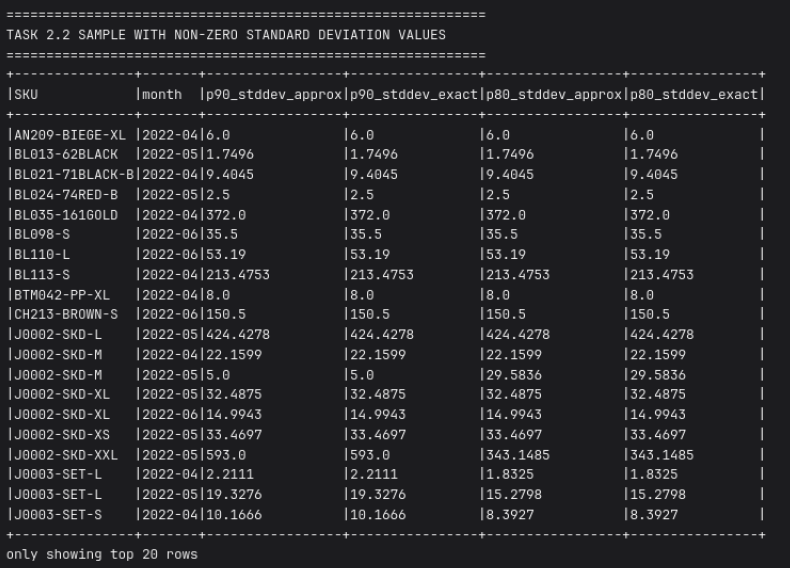
\includegraphics[width=0.9\textwidth]{img/2-2/benchmark.png}
    \caption{Kết quả đo hiệu năng thời gian chạy giữa hai phương pháp}
    \label{fig:task2_2_benchmark}
\end{figure}

\begin{figure}[H]
    \centering
    
\includegraphics[width=0.9\textwidth]{img/2-2/output_preview.png}
    \caption{Một phần nội dung tệp Parquet kết quả đầu ra \texttt{Task\_2-2.parquet}}
    \label{fig:task2_2_output_preview}
\end{figure}


%================================================
% CONCLUSION
%================================================
\section{Kết luận}

\textbf{Tổng kết kết quả.} Điền tóm tắt các kết quả chính của bốn task, bao gồm file output đã tạo, định dạng và trạng thái kiểm chứng.

\textbf{Đánh giá tính đúng.} Điền nhận xét tổng quan về cách nhóm kiểm tra correctness: sample thủ công, schema validation, đọc lại CSV/Parquet, và đối chiếu các điều kiện lọc quan trọng.

\textbf{Đánh giá hiệu năng.} Điền nhận xét chung về hiệu năng: MapReduce phù hợp với các bước key-value aggregation; Spark Structured API thuận lợi cho join/aggregation phức tạp; Task 2.2 cần so sánh chi phí giữa approximate và exact percentile.

\textbf{Khó khăn và hướng cải thiện.} Điền các khó khăn khi xử lý dữ liệu thiếu/null, parse ngày, promotion ids, tie-breaking và partitioning. Nếu có hướng cải thiện, nêu ngắn gọn như bổ sung test tự động, chuẩn hóa schema tốt hơn hoặc tối ưu số partition.


\section{Phụ lục}


\subsection{Source code và Demo}
\begin{itemize}
    \item Link Dataset/Output: \href{https://drive.google.com/drive/folders/106v6y8GMyYHtOZLone474yRZgOjSoNSC?usp=sharing}{Drive}
    \item Source code được nộp trực tiếp trong thư mục \texttt{src} của gói bài làm.
\end{itemize}

% References
\input{ref/ref}








\end{document}
